\documentclass[a4paper]{article}

%====================== PACKAGE ======================

\usepackage[french]{babel}
\usepackage[utf8x]{inputenc}
\usepackage{float}
\usepackage{amsmath}
\usepackage{graphicx}
\usepackage[colorinlistoftodos]{todonotes}
\usepackage{url}
\usepackage{hyperref}
\usepackage{array}
\usepackage{tabularx}
\usepackage{setspace}
\usepackage{abstract}
\usepackage[T1]{fontenc}
\usepackage[top=2cm, bottom=2cm, left=2cm, right=2cm]{geometry}
\usepackage{subfig}
\usepackage{multirow}
\usepackage{svg}
% Définir une nouvelle colonne pour centrer le texte verticalement
\newcolumntype{P}[1]{>{\raggedright\arraybackslash}p{#1}} % Alignement à gauche
\usepackage{listings}   
\usepackage{color}

\definecolor{dkgreen}{rgb}{0,0.6,0}
\definecolor{gray}{rgb}{0.5,0.5,0.5}
\definecolor{mauve}{rgb}{0.58,0,0.82}
\usepackage{courier} %% Sets font for listing as Courier.
\usepackage{listings, xcolor}
\lstset{%
  tabsize = 4, %% set tab space width
  showstringspaces = false, %% prevent space marking in strings, string is defined as the text that is generally printed directly to the console
  commentstyle = \color{dkgreen}, %% set comment color
  keywordstyle = \color{blue}, %% set keyword color
  stringstyle = \color{orange}, %% set string color
  rulecolor = \color{black}, %% set frame color to avoid being affected by text color
  basicstyle = \small\ttfamily, %% set listing font and size
  breaklines = true, %% enable line breaking
  numberstyle = \tiny,
}


%====================== INFORMATION ET REGLES ======================

\setcounter{secnumdepth}{4}
\setcounter{tocdepth}{4}

\hypersetup{							% Information sur le document
pdfauthor = {Simon Perret},			% Auteurs
pdftitle = {Nom du Projet - Sujet du Projet},			% Titre du document
pdfsubject = {Mémoire de Projet},		% Sujet
pdfstartview={FitH}}					% ajuste la page à la largueur de l'écran

%======================== DEBUT DU DOCUMENT ========================

\begin{document}

%régler l'espacement entre les lignes
\newcommand{\HRule}{\rule{\linewidth}{0.5mm}}

%page de garde
\begin{titlepage}
\begin{center}

% Upper part of the page. The '~' is needed because only works if a paragraph has started.

\includegraphics[width=0.5\textwidth]{./logo.png}~\\[2.5cm]

\textsc{\LARGE INSA de Lyon}\\[0.5cm]
\textsc{\Large Département Informatique}\\[0.5cm]
\textsc{\LARGE Développement d'applications pour les SI}\\[1.5cm]

% Title
\HRule \\[0.4cm]

{\huge \bfseries TP DASI \\
\textsc{Instruct'IF} \\[0.4cm] }

\HRule \\[1.5cm]

% Author and supervisor
\begin{minipage}{0.4\textwidth}
\begin{flushleft} \large
\emph{Auteurs:}\\
Binôme B3423 :\\
Saad \textsc{ElGhissassi}\\
Simon \textsc{Perret}\\
\end{flushleft}
\end{minipage}
\begin{minipage}{0.4\textwidth}
\begin{flushright} \large
\emph{Professeurs:} \\
Mme. \textsc{Tchounikine}\\
Mme. \textsc{Servigne}\\
M. \textsc{Duclos}\\
M. \textsc{Gripay}\\
\end{flushright}
\end{minipage}

\vspace{2.5cm}
\setcounter{tocdepth}{1}
\tableofcontents
% Bottom of the page
\vfill
{\large \today}

\end{center}
\end{titlepage}


\setcounter{page}{1}

%====================== INCLUSION DES PARTIES ======================

%introduction
\section*{Introduction}
\addcontentsline{toc}{section}{Introduction}
La plateforme INSTRUCT’IF se présente comme une solution numérique innovante destinée à faciliter l'aide aux devoirs pour les élèves de niveau collège et lycée. Ce projet incarne une plateforme dynamique facilitant la connexion entre des élèves en quête de soutien académique et des intervenants qualifiés prêts à offrir leur expertise bénévolement.
\newline
\\
L'une des principales forces d’INSTRUCT’IF réside dans sa facilité d'utilisation, offrant aux élèves un moyen rapide et intuitif de demander de l'aide. En quelques clics, une demande de soutien est soumise et traitée aboutissant à l'assignation automatique d'un intervenant approprié. Un système de visioconférence intégré, assurant des sessions de tutorat interactives et adaptées aux besoins spécifiques de chaque élève, renforce l'accessibilité et l'efficacité des soutiens scolaires proposés par la plateforme, ce qui favorise une expérience d'apprentissage immersive et personnalisée, permettant aux élèves de surmonter leurs difficultés scolaires dans un environnement stimulant et sécurisant. \newline
\\
Ce rapport détaillera les fonctionnalités clés d’INSTRUCT’IF en mettant l’accent sur les processus qui ont permis sa conception.



\section{Description des cas d'usage}

\begin{figure}[H]
    \centering
    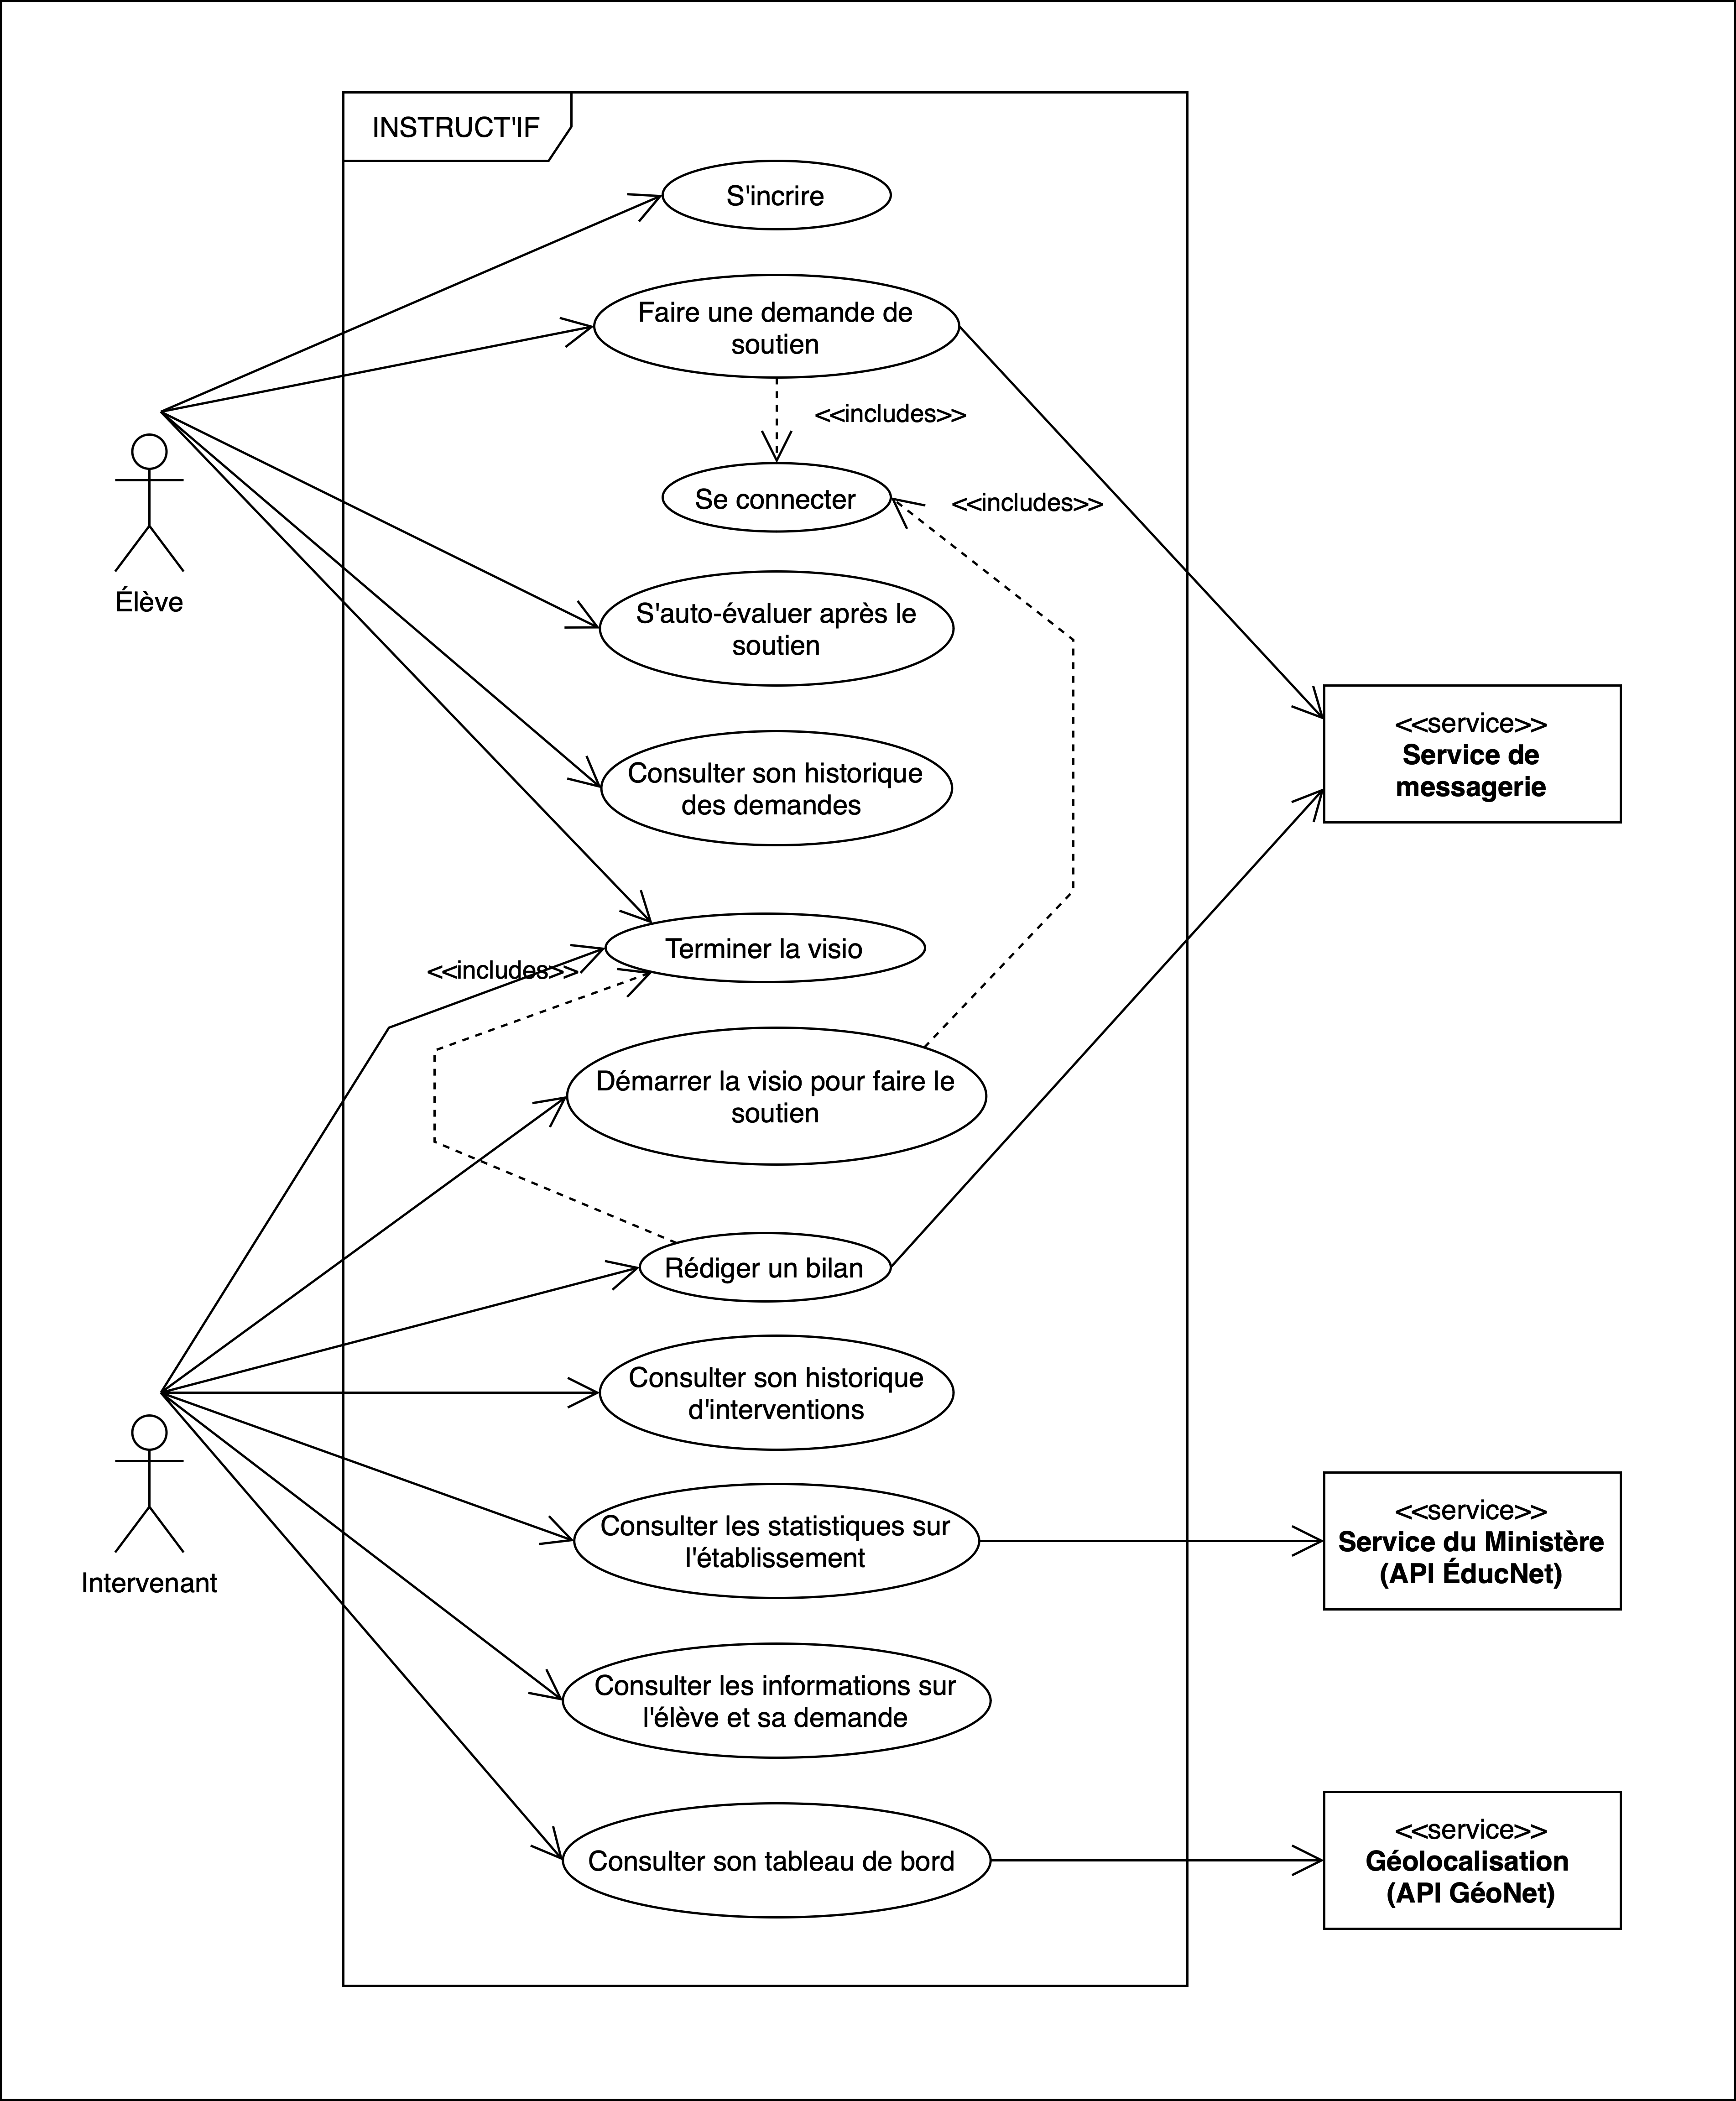
\includegraphics[width=8cm]{usercase.png}
    \caption{Diagramme des cas d'utilisation de l'application Instruct'IF}
    \label{usecase}
\end{figure}

\subsection{Description du cahier des charges}
\begin{description}
    \item[Elève] 
    Sur INSTRUCT'IF, l'élève s'inscrit en indiquant ses données et le code de son établissement pour créer un profil. Après inscription, il se connecte pour une demande de soutien, choisissant une matière et exposant sa difficulté. La plateforme sélectionne alors l'intervenant approprié en fonction du niveau et de la disponibilité. En cas d'indisponibilité, un email invite à renouveler la demande. Sinon, la visioconférence démarre. L'élève évalue à l'issue du soutien la qualité de ce dernier, et reçoit un bilan par mail. Il a aussi accès à l'historique des sessions pour consulter les retours des intervenants.\newline
    \item[Intervenant] Les intervenants d'INSTRUCT'IF, étudiants, enseignants ou bénévoles, aident collégiens et lycéens. Inscrits sur la plate-forme, ils peuvent des demandes de soutien par SMS. Les intervenants sont sélectionnés par un algorithme favorisant ceux ayant le moins contribué. Les intervenants sont ouverts à toutes les matières, mais ils indiquent au préalable les classes des élèves qu'ils acceptent d'accompagner. Après une session, ils rédigent un bilan et peuvent voir des statistiques sur leur tableau de bord, comme le nombre d'élèves, d'interventions et la satisfaction moyenne.
\end{description}

\subsection{Diagramme des cas d'utilisation}
Le diagramme de la figure~\ref{usecase} dépeint l'interface de la plateforme INSTRUCT'IF, détaillant les fonctionnalités pour les élèves et les intervenants. Les élèves s'enregistrent, demandent des soutiens, participent à des visioconférences et suivent leurs progrès. Les intervenants gèrent les demandes, historiques et rédigent des bilans. Des API externes enrichissent la plateforme avec des services de messagerie et de géolocalisation.

\section{Modèle du domaine}

\begin{figure}[H]
    \centering
    \fbox{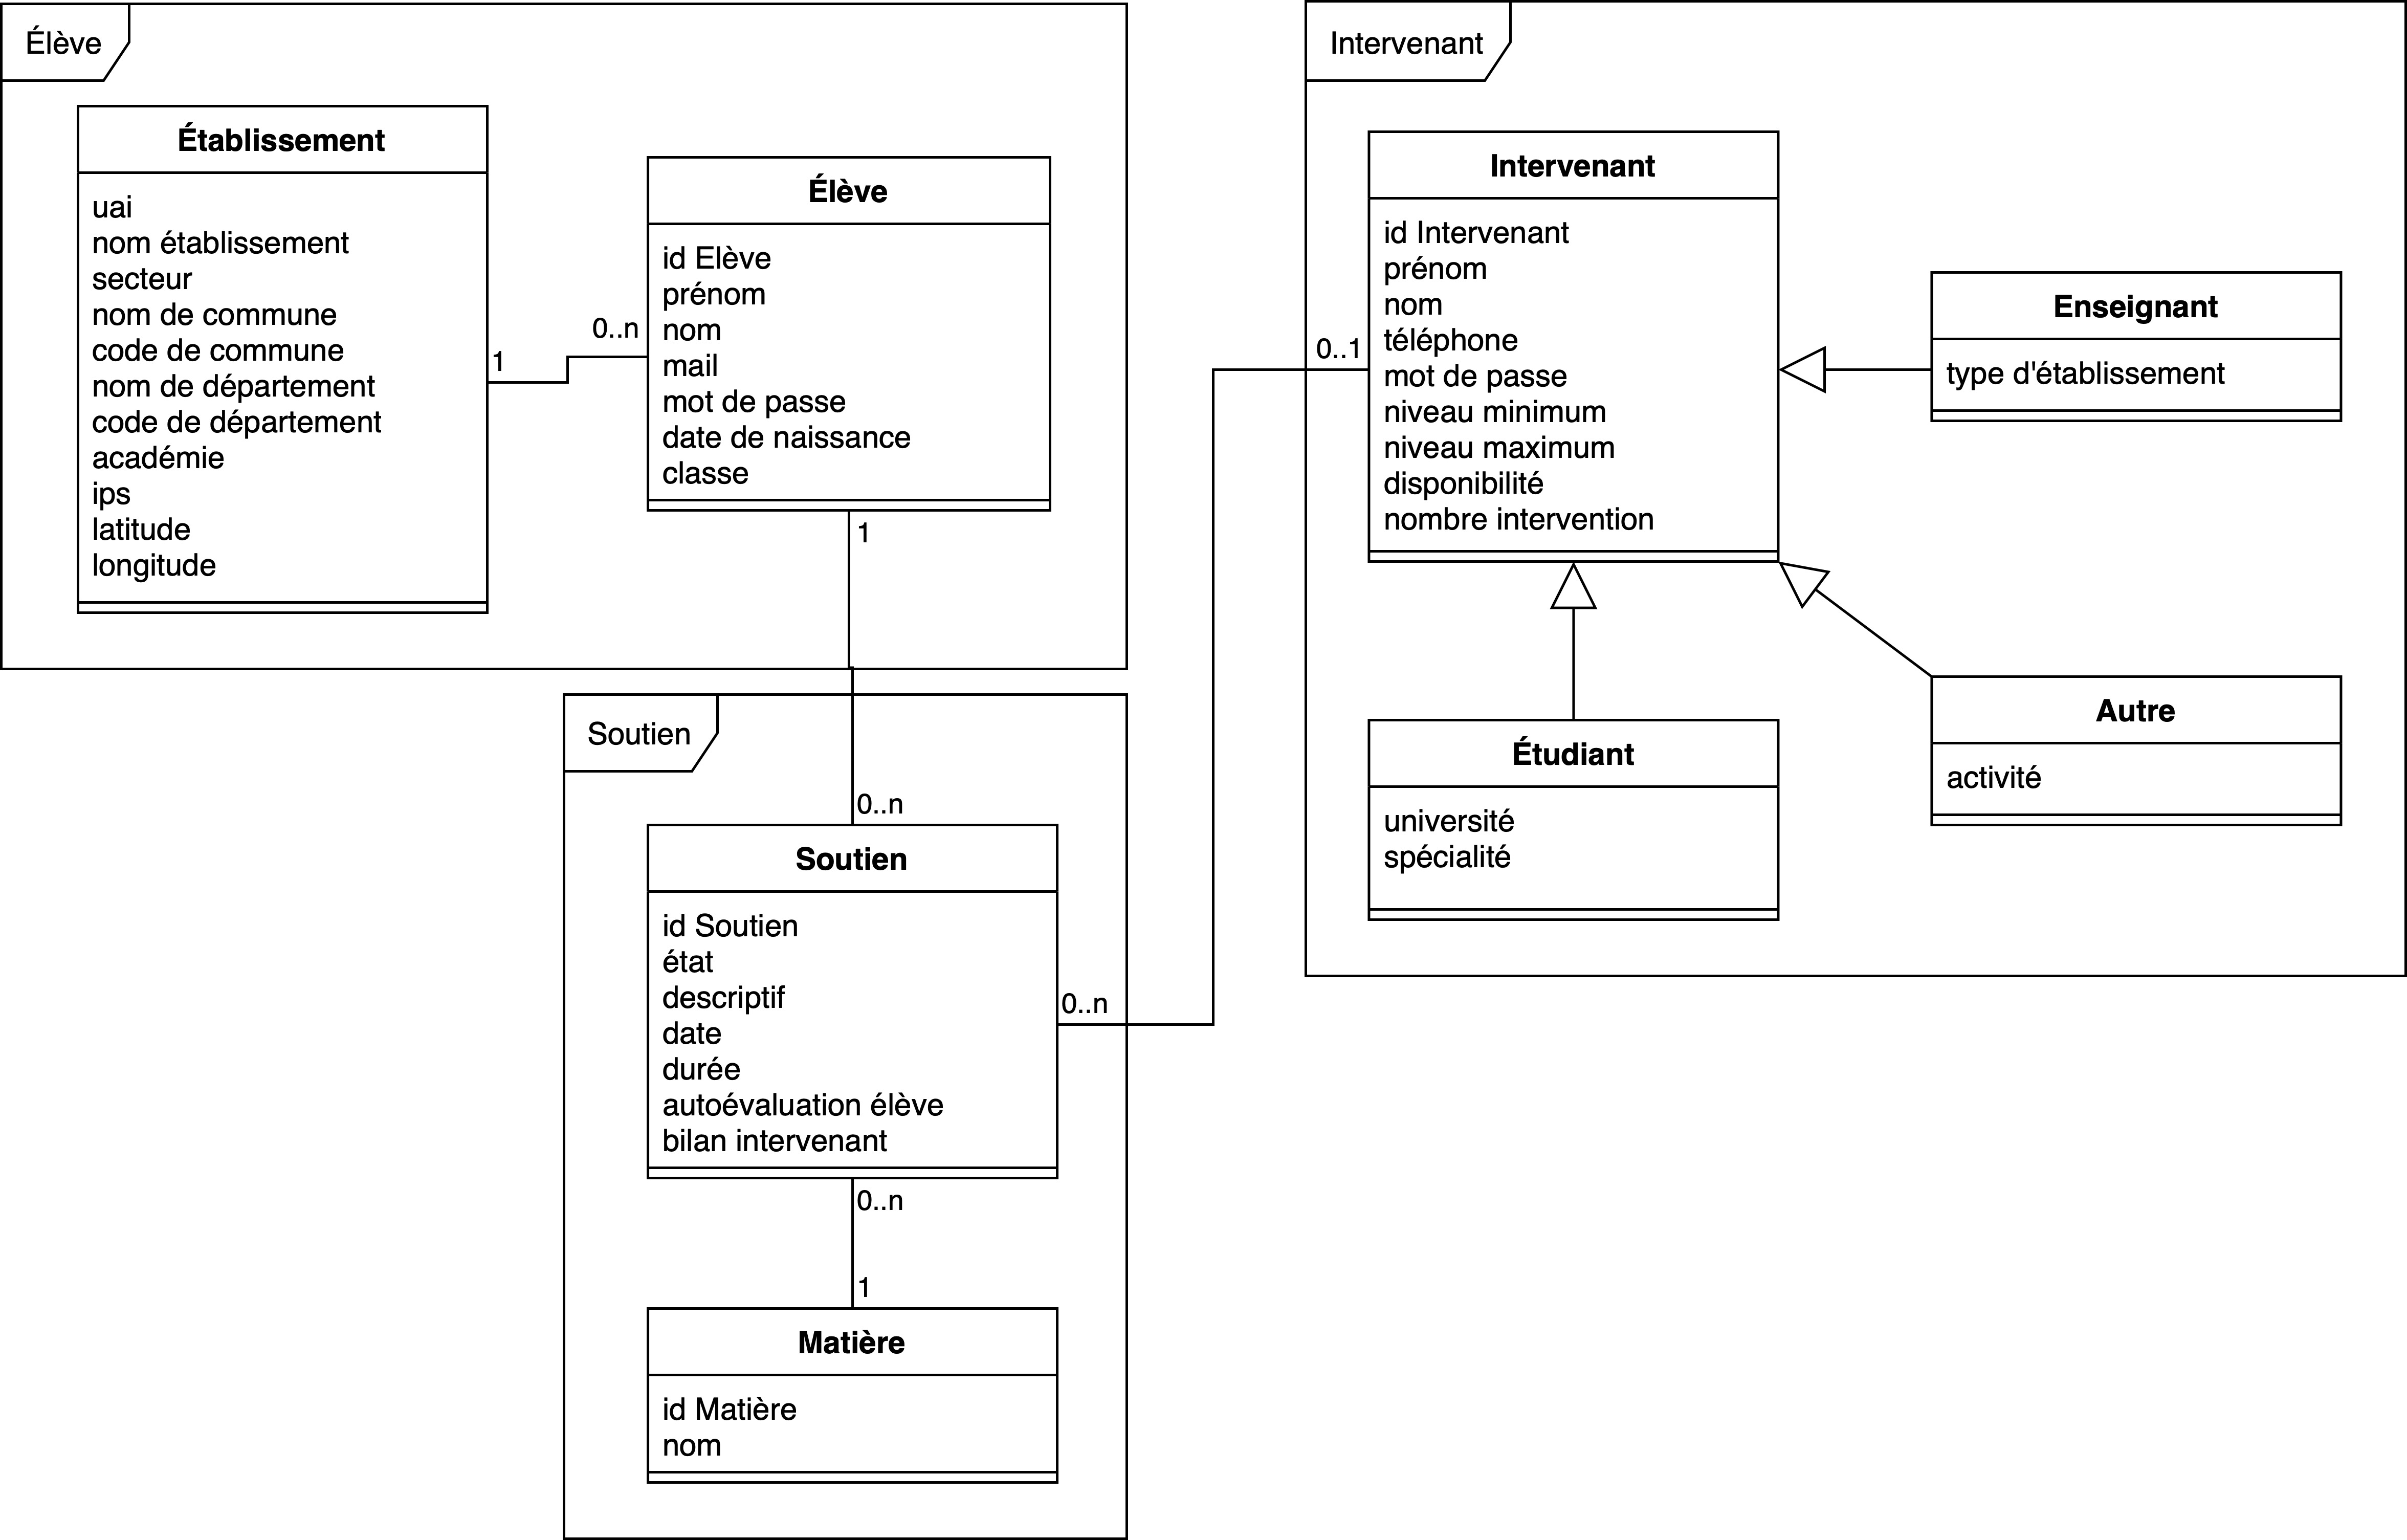
\includegraphics[width=10cm]{modele.jpg}}
    \caption{Modèle Conceptuel de Données (MCD) d'Instruct'IF}
    \label{modele}
\end{figure}

Le modèle du domaine d'INSTRUCT'IF est conçu pour gérer efficacement les relations entre les élèves, les intervenants et les soutiens scolaires. Il s'appuie sur une structure de base de données relationnelle, utilisant l'héritage et les relations entre entités pour modéliser les interactions du système. Voici une description de son architecture principale et des entités clés :

\subsection{Entités principales}
\begin{description}
    \item[Elève] Cette entité représente les utilisateurs élèves de l'application. Chaque élève est caractérisé par  ses attributs dont un identifiant (unique et généré automatiquement), son mail (unique) ou encore son établissement auquel il est rattaché. L'association avec l'établissement est gérée via une relation ManyToOne.\newline
    \item[Intervenant] Base de l'héritage pour les intervenants, cette entité contient les attributs communs à tous les types d'intervenants dont un identifiant (unique et généré automatiquement) ou encore son téléphone (unique également). L'héritage est implémenté via l'annotation \texttt{@Inheritance(strategy = InheritanceType.JOINED)}, permettant de dériver d'autres types d'intervenants tout en partageant la même table de base : \texttt{Etudiant} ayant les attributs université et spécialité, \texttt{Enseignant} ayant l'attribut du type d'établissement et \texttt{AutreIntervenant} avec un attribut précisant leur activité principale.
\newline
    \item[Soutien]Cette entité représente une session de soutien scolaire. Elle inclut entre autres l'état du soutien : \texttt{EN\_ATTENTE}, \texttt{EN\_VISIO}, \texttt{TERMINE} et des relations ManyToOne avec les entités Matiere, Eleve et Intervenant.
\newline
\item[Matiere]Représente les différentes matières enseignées. Chaque matière est caractérisée par un identifiant unique et un nom.
\newline
\item[Etablissement]Décrit les établissements scolaires. Chaque établissement a entre autres un identifiant unique (UAI) et ses coordonnées géographiques (latitude et longitude) récupérées grâce à l'API.
\newline
\end{description}


\subsection{Diagramme des classes}

Le diagramme de la figure~\ref{modele} montre l'agencement des données dans INSTRUCT'IF, reliant élèves, établissements et intervenants. Il souligne l'inscription des élèves, la gestion des soutiens et l'assignation des intervenants par spécialité. Ce modèle soutient la coordination des activités éducatives sur la plateforme.

\section{Description des IHM}
\subsection{Enchaînement des fenêtres}

\begin{figure}[H]
    \centering
    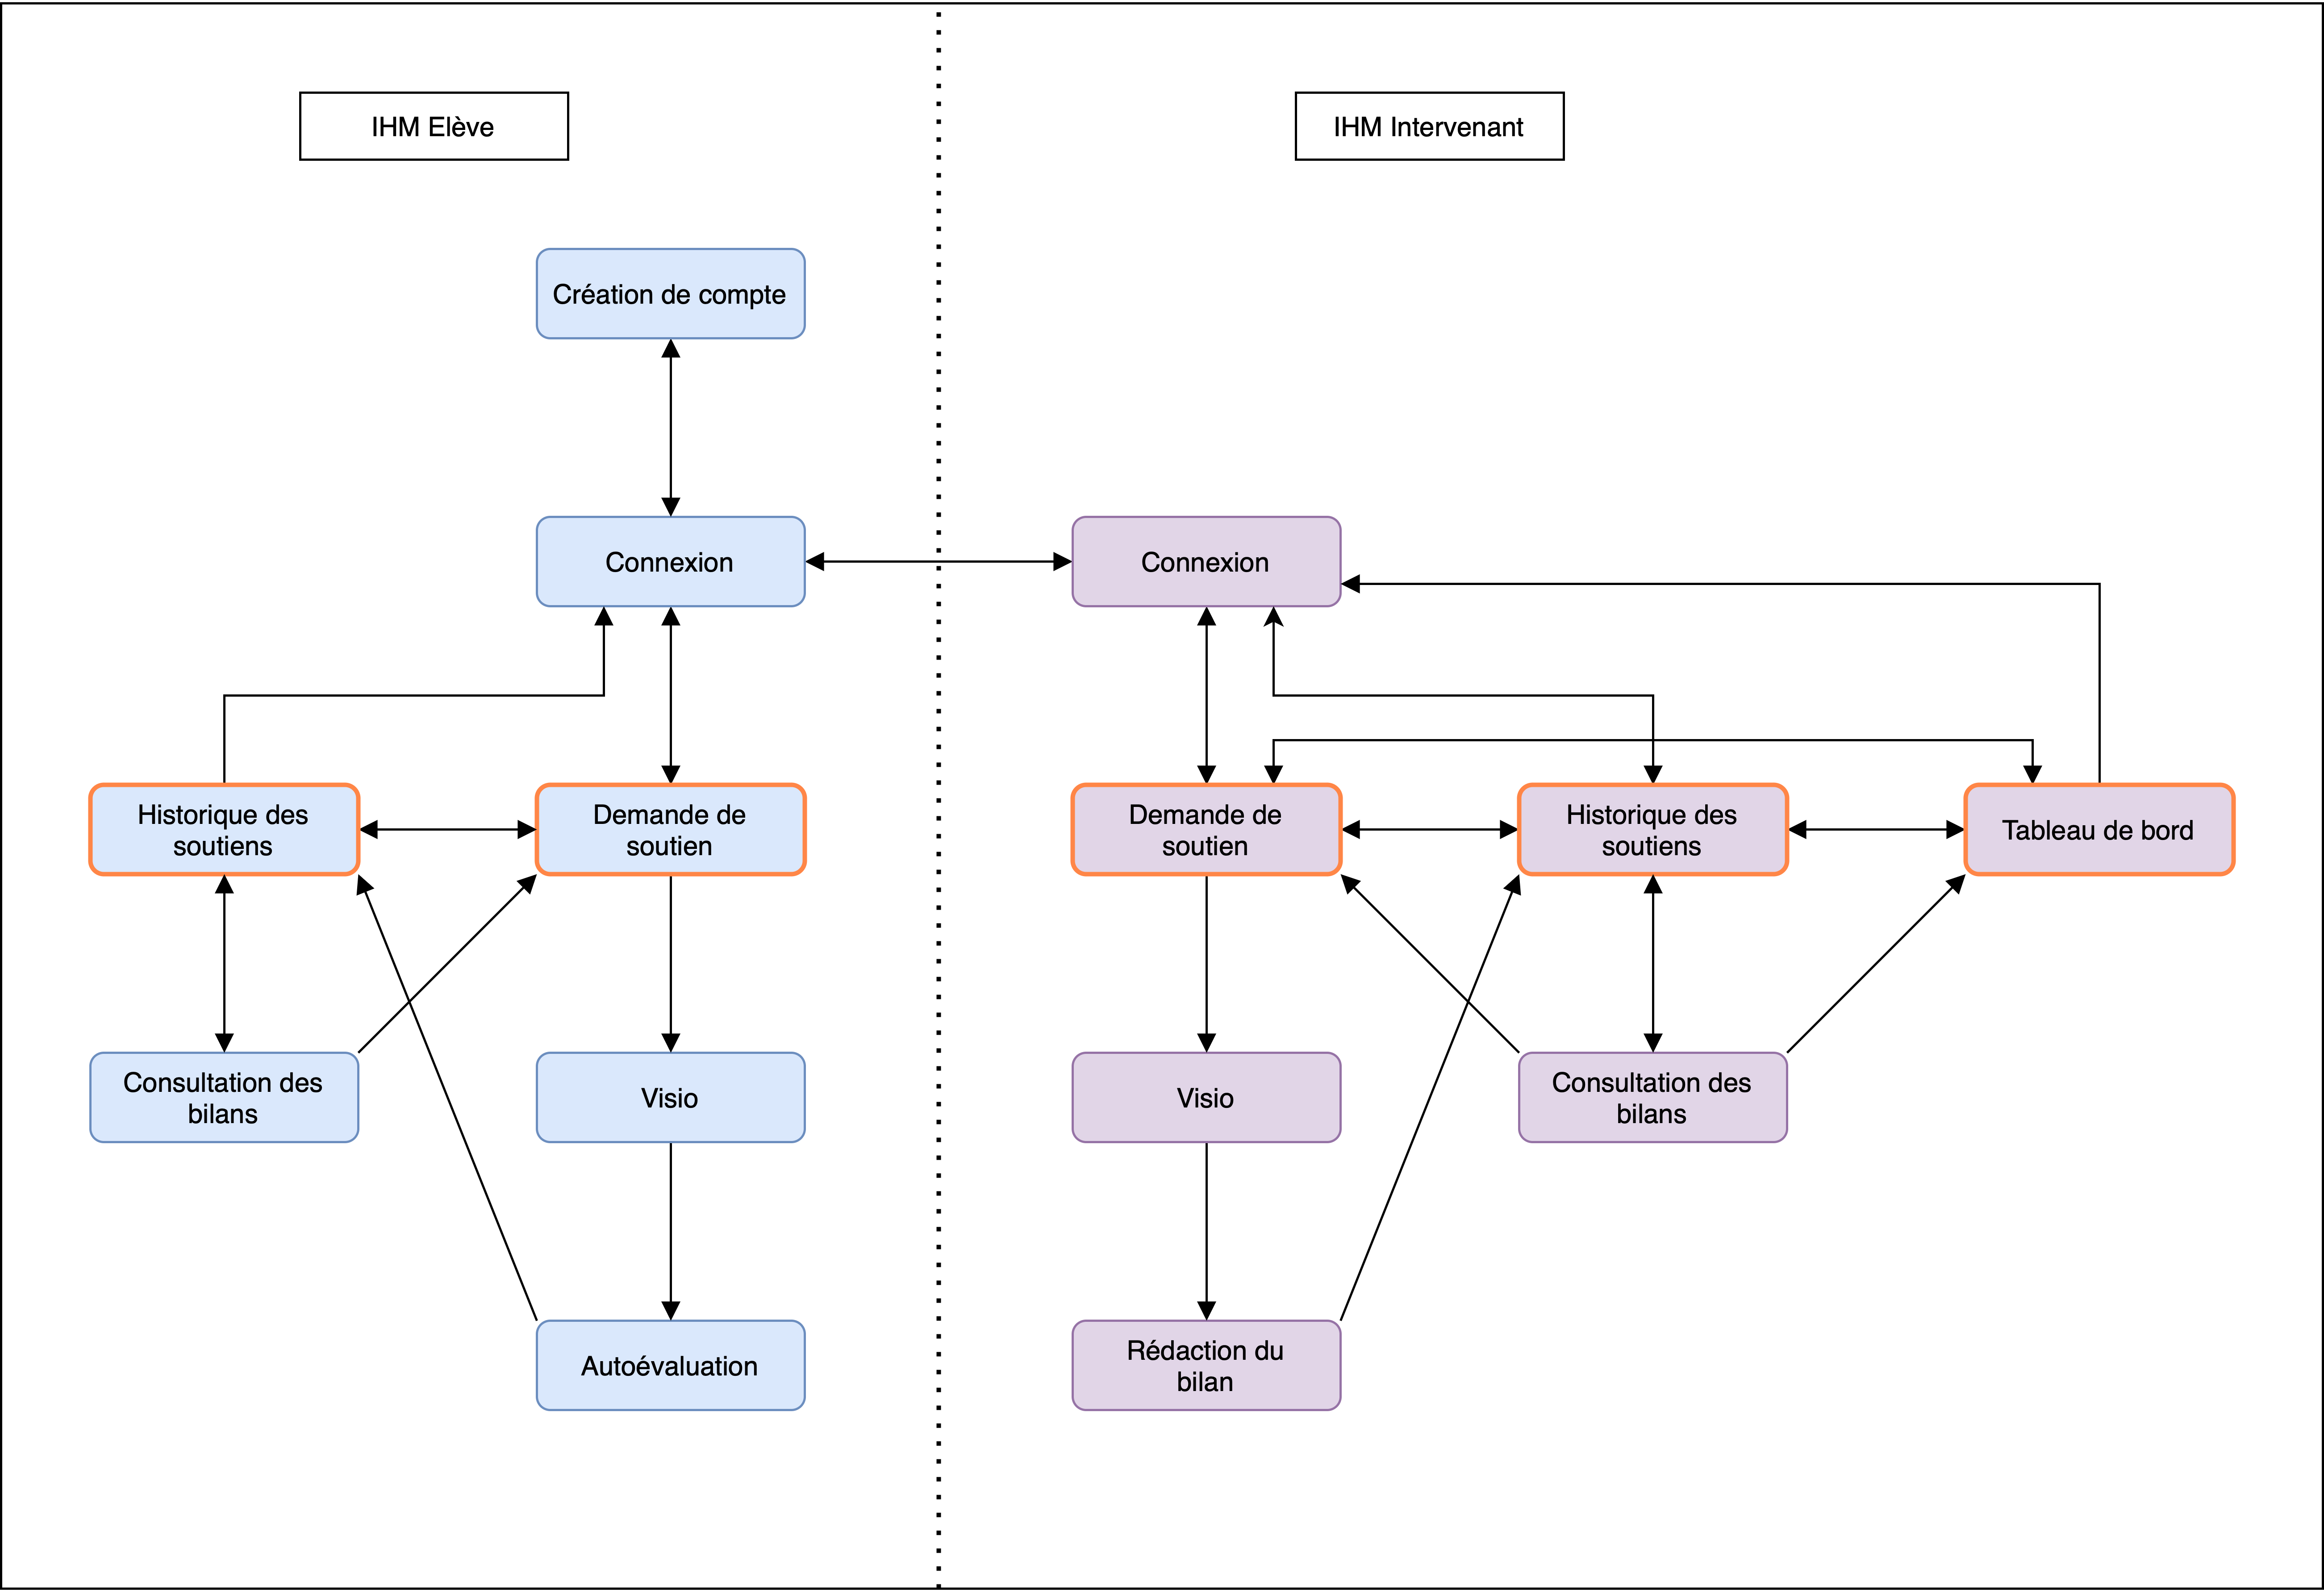
\includegraphics[width=10cm]{edf.png}
    \caption{Diagramme des enchaînements de fenêtres l'application Instruct'IF}
\end{figure}

Nous avons conçu l’interface d’INSTRUCT’IF pour qu’elle soit intuitive. Ainsi, les flux d'actions pour les élèves et pour les intervenants sont clairement définis, permettant une navigation fluide et une expérience utilisateur optimisée. Cela assure que les utilisateurs, qu'ils soient élèves ou intervenants, puissent facilement réaliser les actions clés nécessaires pour l'utilisation de la plateforme INSTRUCT'IF.

L'enchaînement des IHM (Interface Homme-Machine) présenté dans le diagramme ci-dessus montre les flux d'interactions pour les élèves et les intervenants sur la plateforme INSTRUCT'IF.

Les fonctionnalités clés, encadrées en orange, sont intégrées dans le bandeau d'en-tête du site, rendant ces options régulièrement accessibles aux utilisateurs. Pour les élèves, cela comprend la demande de soutien et l'historique des soutiens. Les intervenants ont un accès facile à la demande de soutien, à l'historique des soutiens, ainsi qu'à leur tableau de bord. Ces IHM essentielles sont complétées par des fonctionnalités telles que la visioconférence et l'autoévaluation pour les élèves, ainsi que la rédaction du bilan pour les intervenants.

\subsection{IHM Communes}
\begin{figure}[H]
    \centering % Centre les figures dans la page
    \begin{minipage}{0.49\textwidth} % Ajuste la largeur du minipage à moins de la moitié de la largeur de la page
        \centering
        \fbox{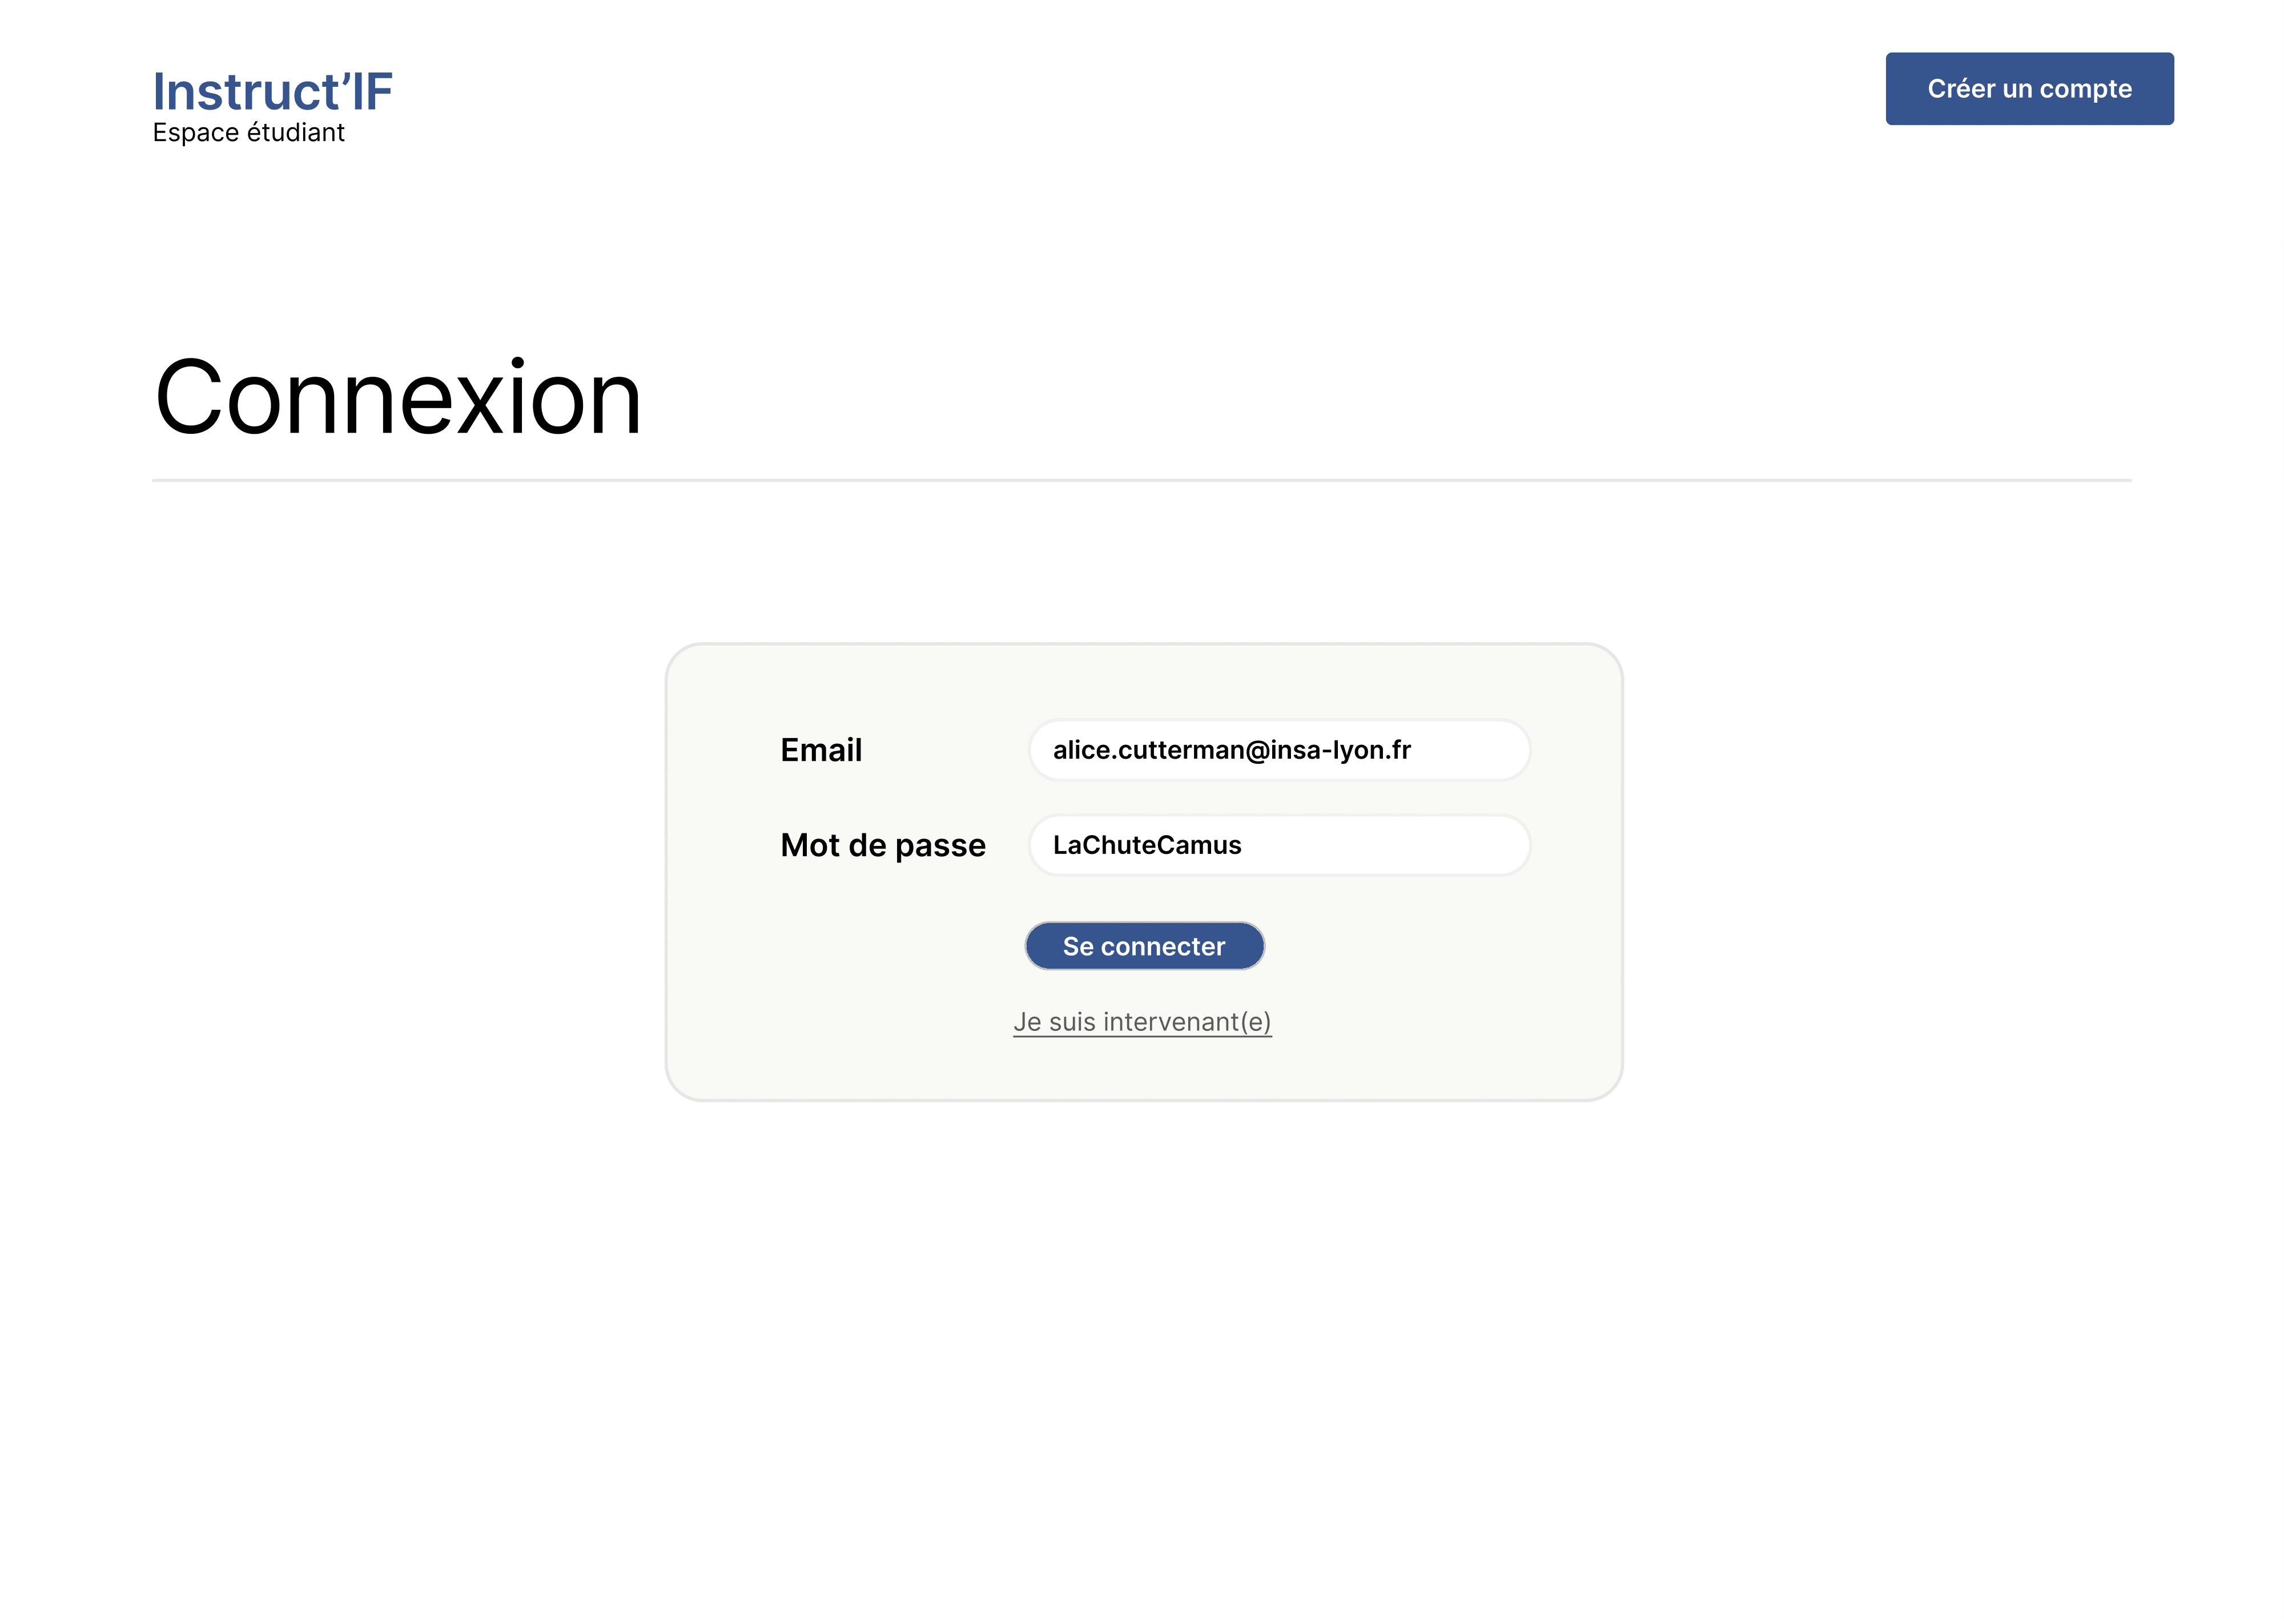
\includegraphics[width=\linewidth]{IHM/loginEleve.png}} % Ajuste la largeur de l'image à moins de la largeur du minipage
        \caption{Fenêtre de connexion (Elève)}
    \end{minipage}\hfill % Ajoute un petit espace entre les deux minipages
    \begin{minipage}{0.49\textwidth} % Identique au premier minipage
        \centering
        \fbox{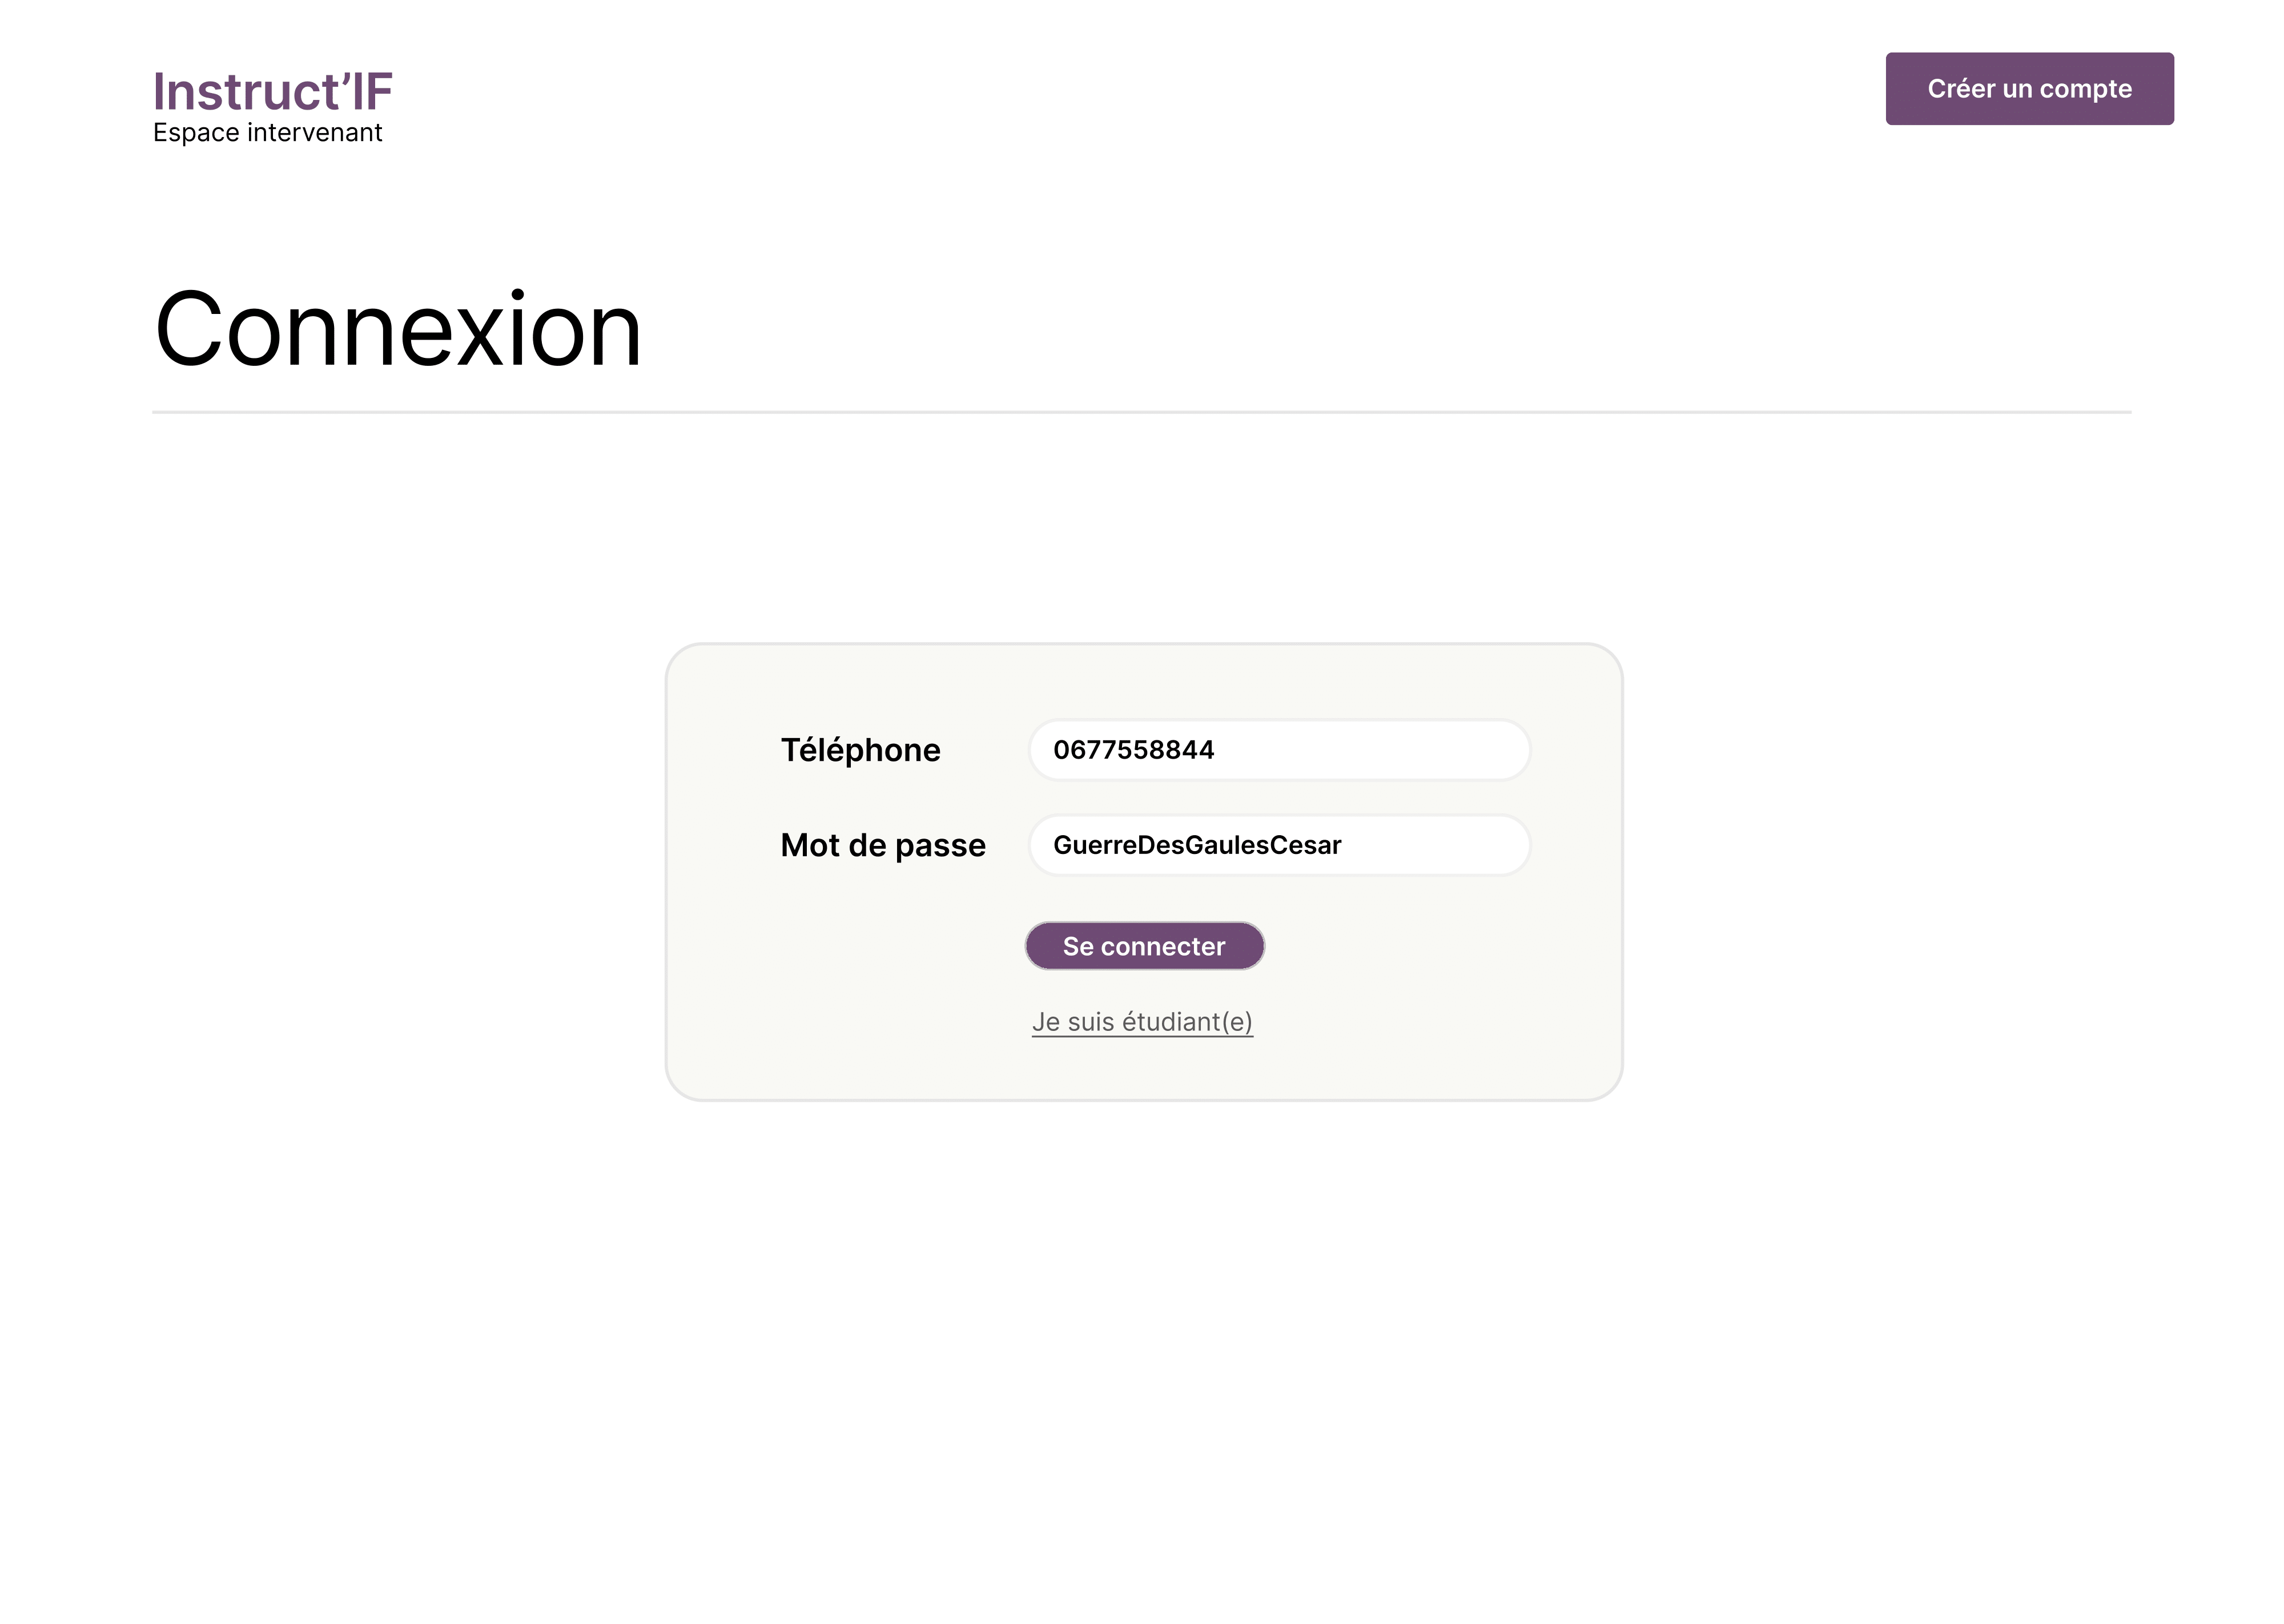
\includegraphics[width=\linewidth]{IHM/loginIntervenant.png}}
        \caption{Fenêtre de connexion (Intervenant)}
    \end{minipage}
\end{figure}

\begin{figure}[H]
    \centering
    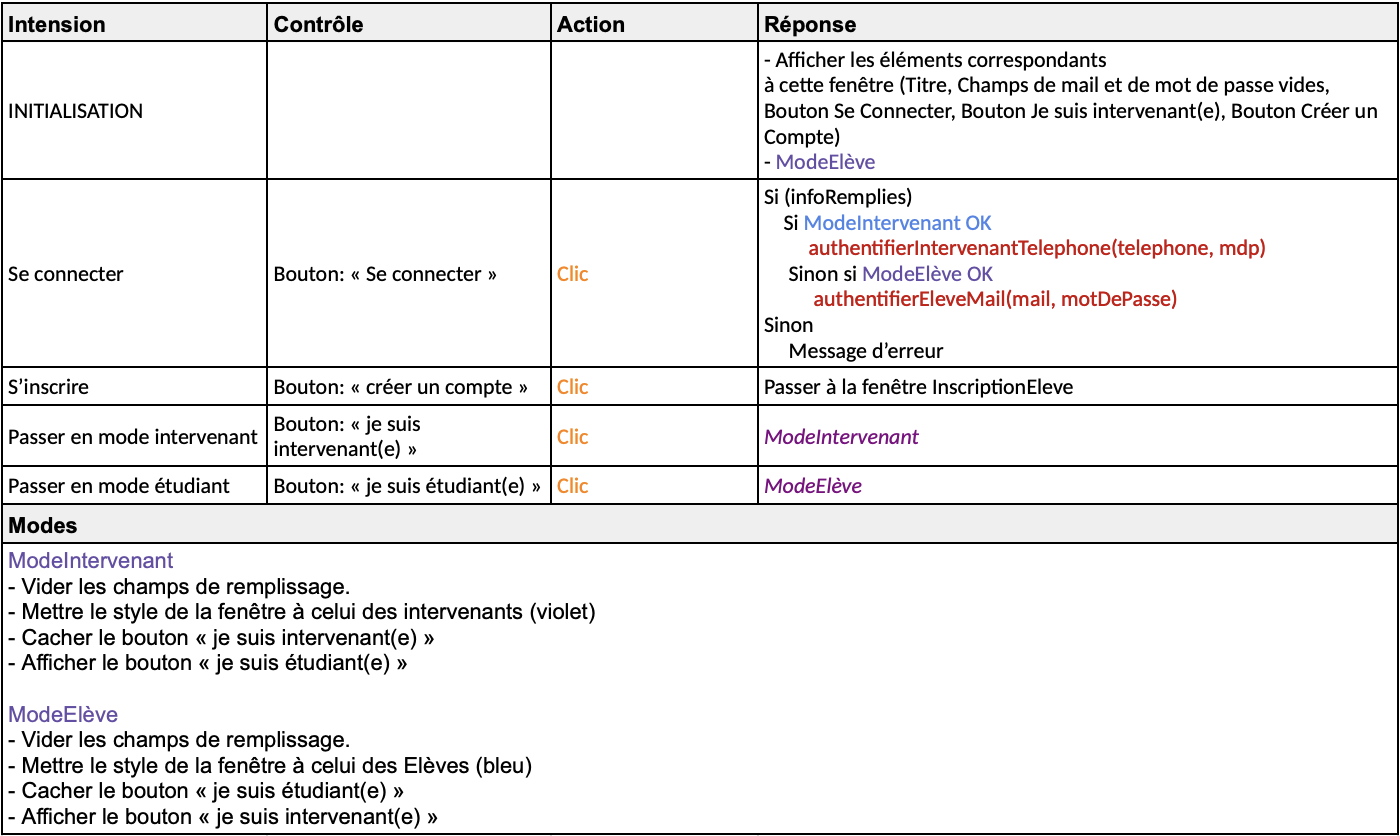
\includegraphics[width=13cm]{ICARS/connexion.png}
    \caption{ICAR+S associé à l'IHM de connexion}
\end{figure}

\begin{figure}[H]
    \centering % Centre les figures dans la page
    \begin{minipage}{0.49\textwidth} % Ajuste la largeur du minipage à moins de la moitié de la largeur de la page
        \centering
        \fbox{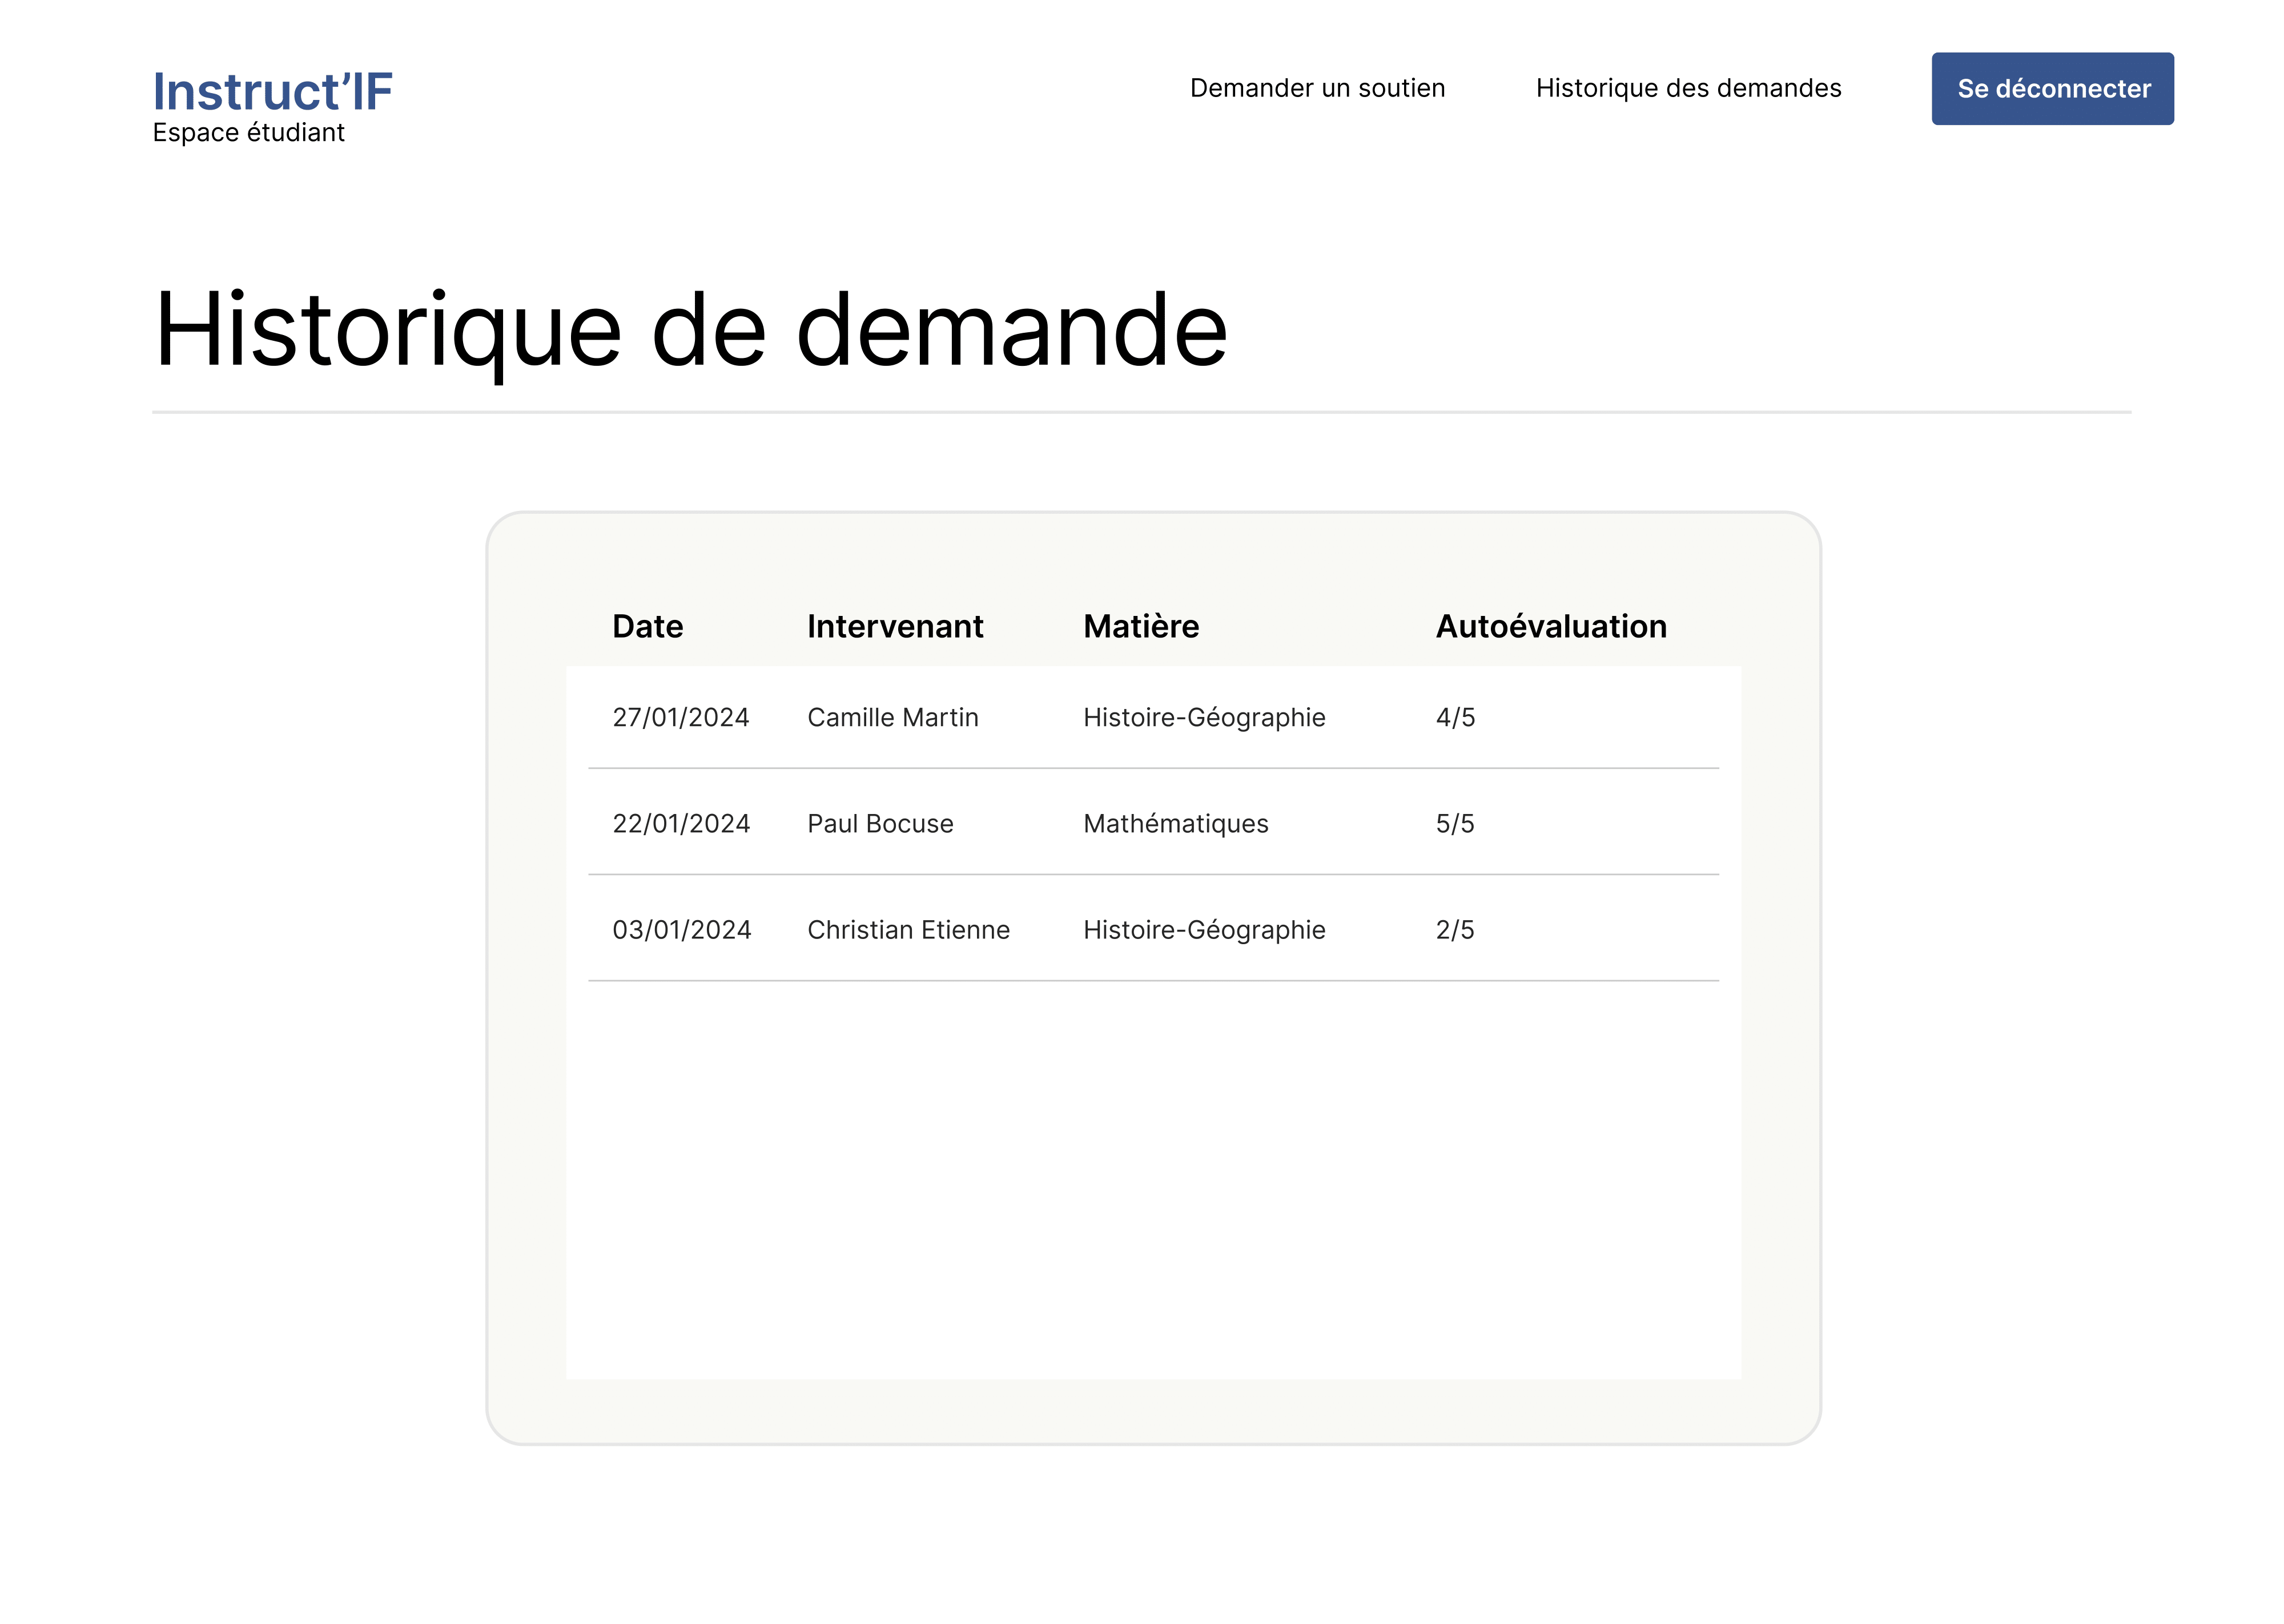
\includegraphics[width=\linewidth]{IHM/historiqueEleve.png}} % Ajuste la largeur de l'image à moins de la largeur du minipage
        \caption{Consultation de l'historique (Elève)}
    \end{minipage}\hfill % Ajoute un petit espace entre les deux minipages
    \begin{minipage}{0.49\textwidth} % Identique au premier minipage
        \centering
        \fbox{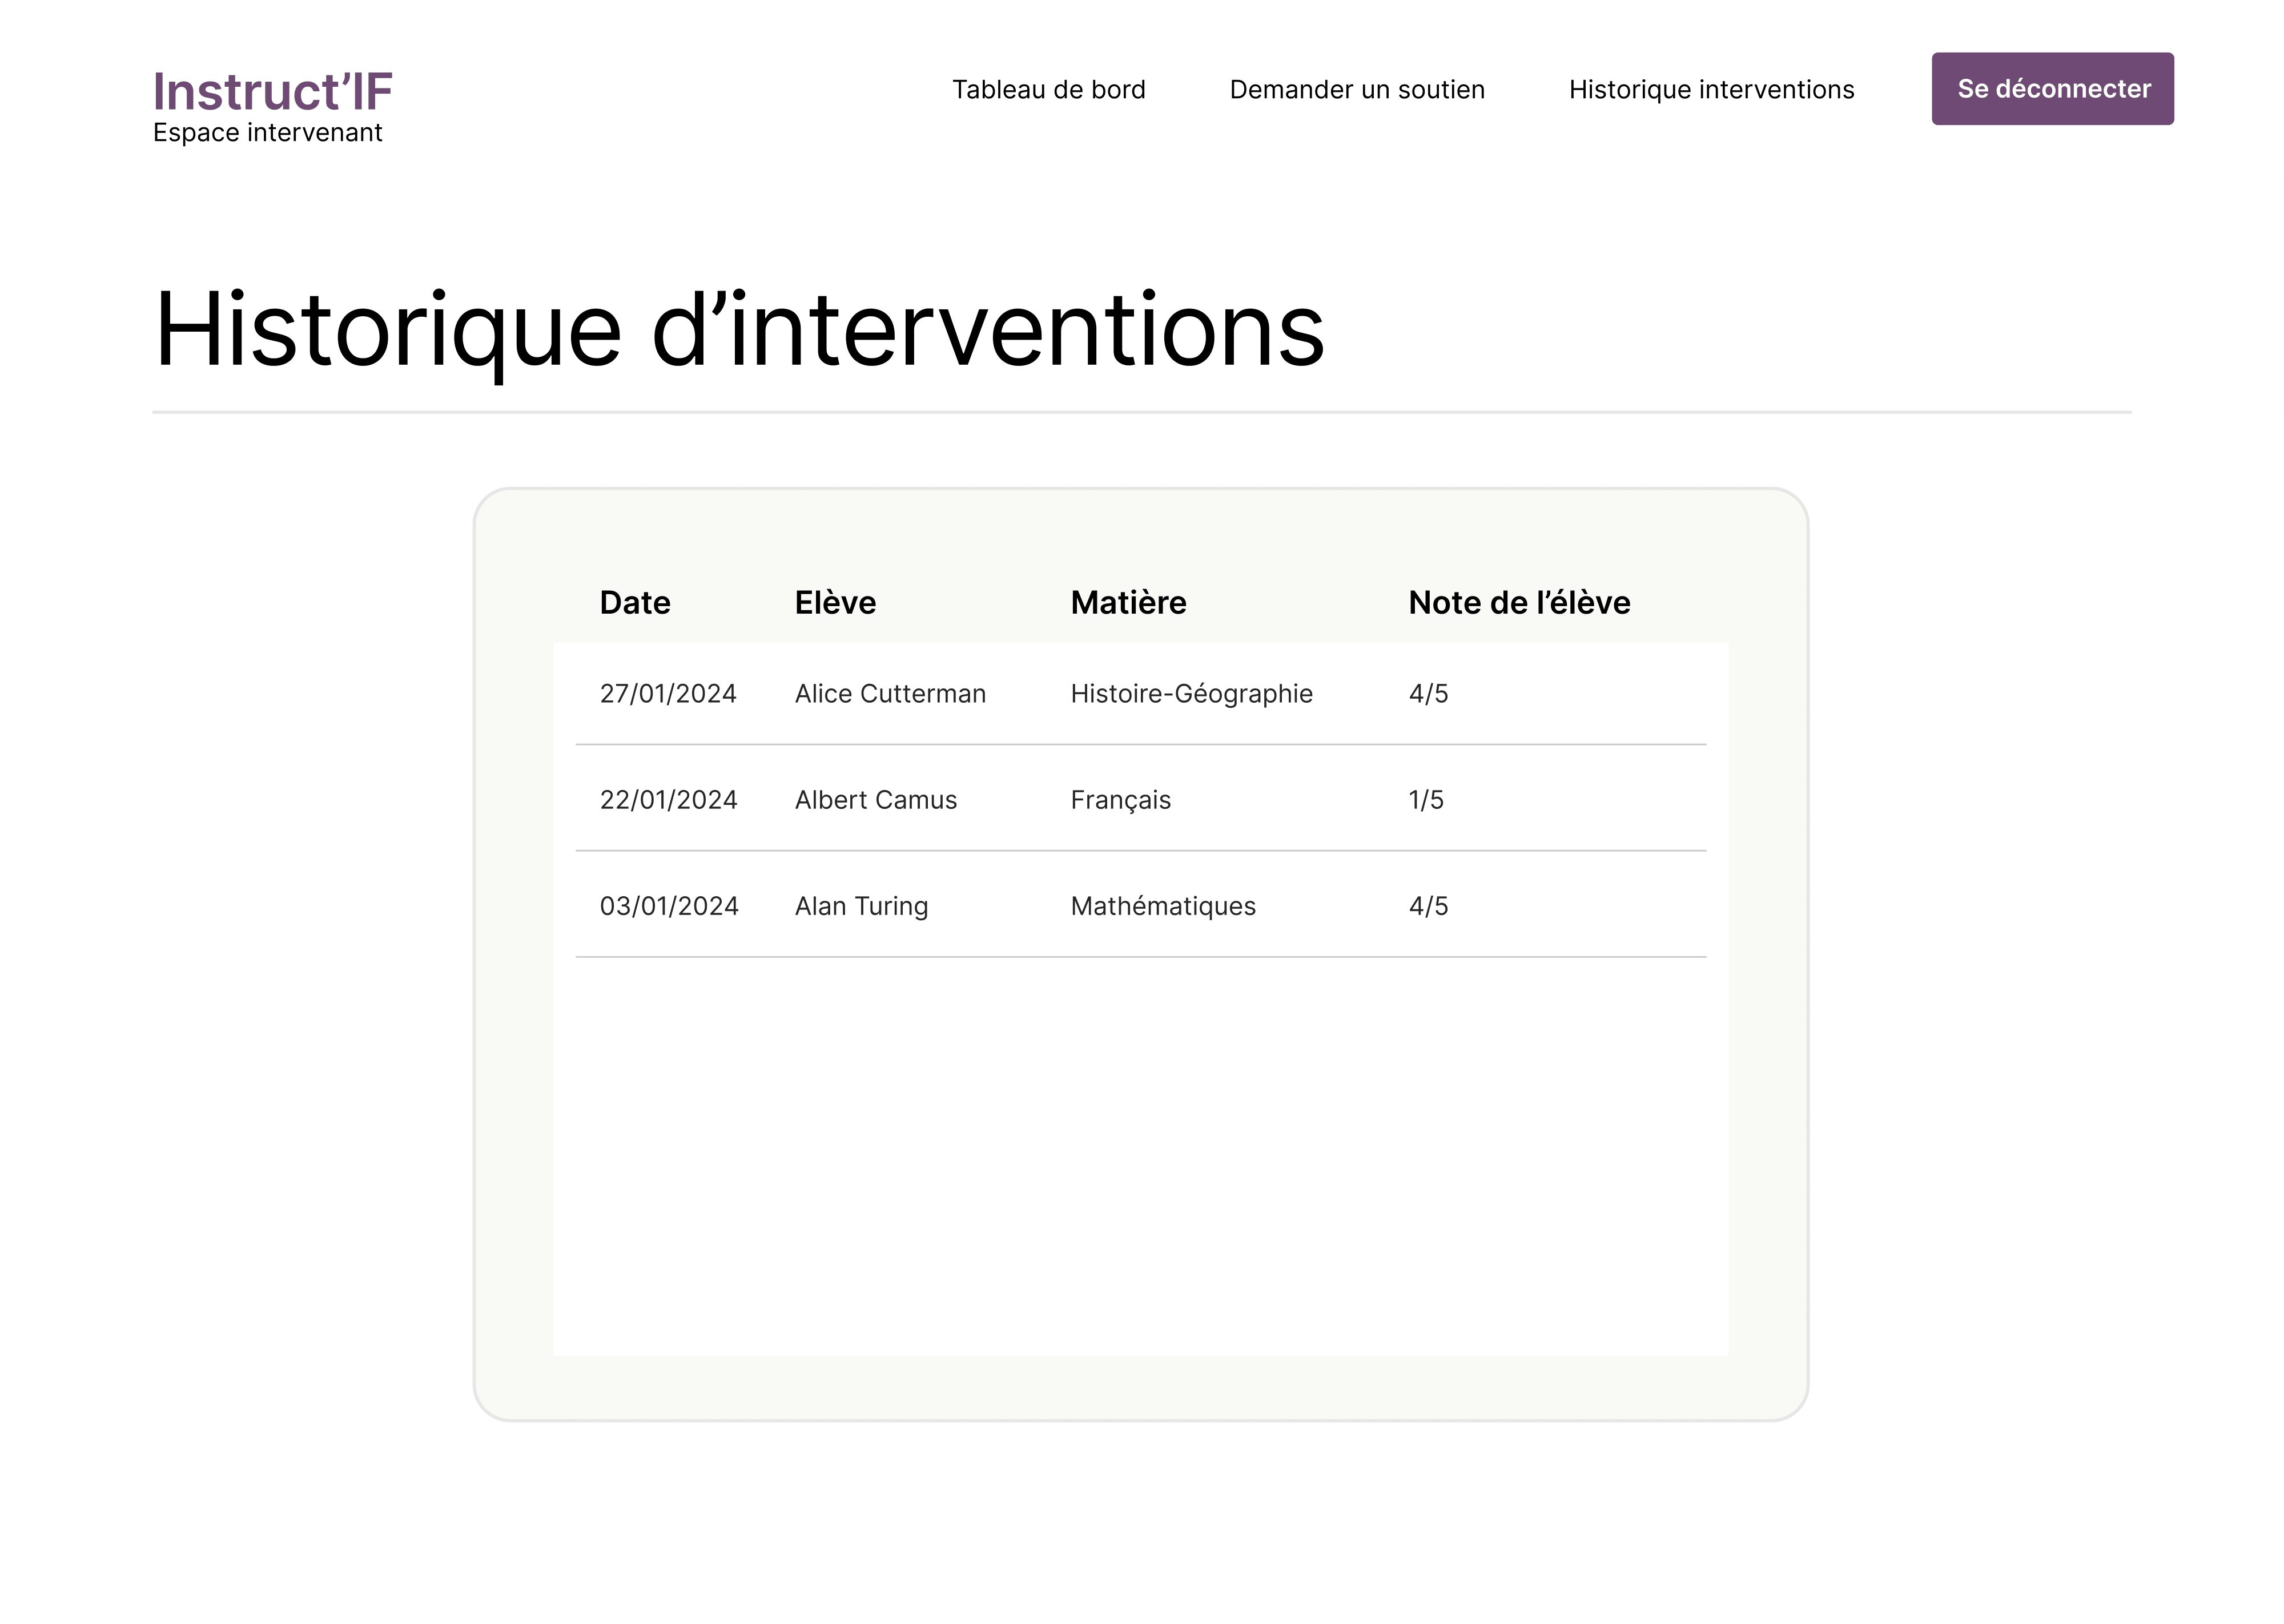
\includegraphics[width=\linewidth]{IHM/historiqueIntervenant.png}}
        \caption{Consultation de l'historique (Intervenant)}
    \end{minipage}
\end{figure}

\begin{figure}[H]
    \centering
    
\includegraphics[width=10cm]{IHM/visio.png}
    \caption{Fenêtre de visioconférence}
\end{figure}

\begin{figure}[H]
    \centering
    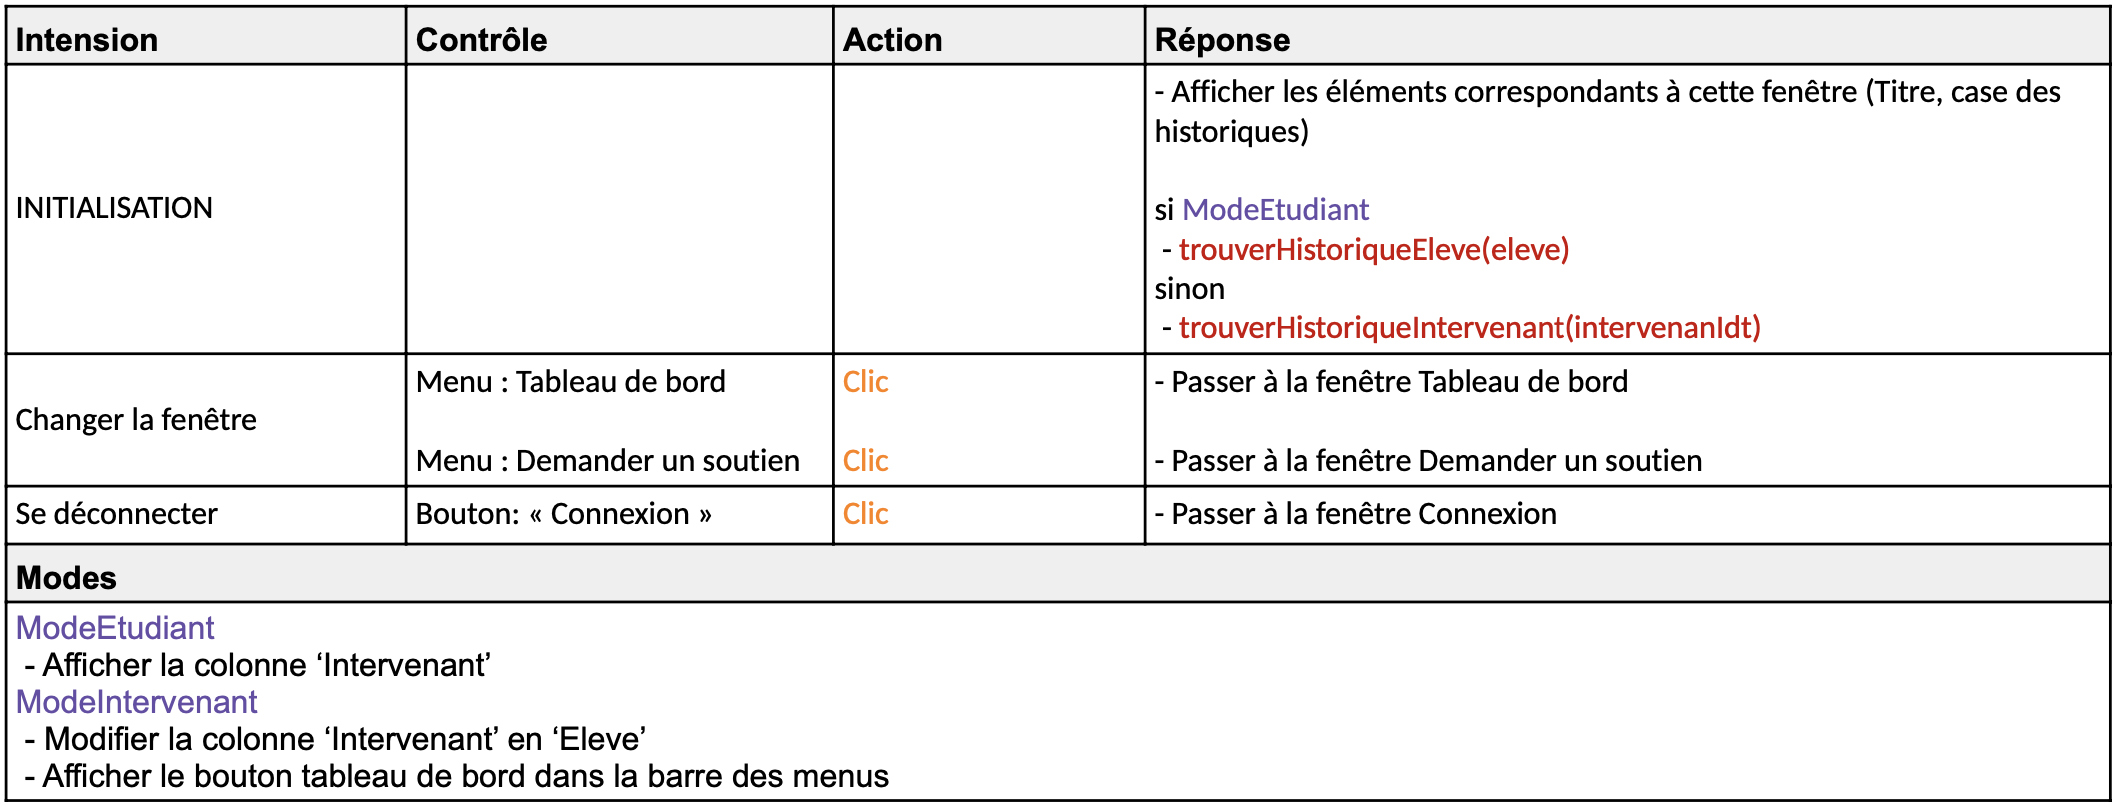
\includegraphics[width=13cm]{ICARS/historique.png}
    \caption{ICAR+S associé à l'IHM de l'historique}
\end{figure}

\begin{figure}[H]
    \centering
    
\includegraphics[width=13cm]{ICARS/visio.png}
    \caption{ICAR+S associé à l'IHM de visioconférence}
\end{figure}

\subsection{IHM Elève}

\begin{figure}[H]
    \centering
    \fbox{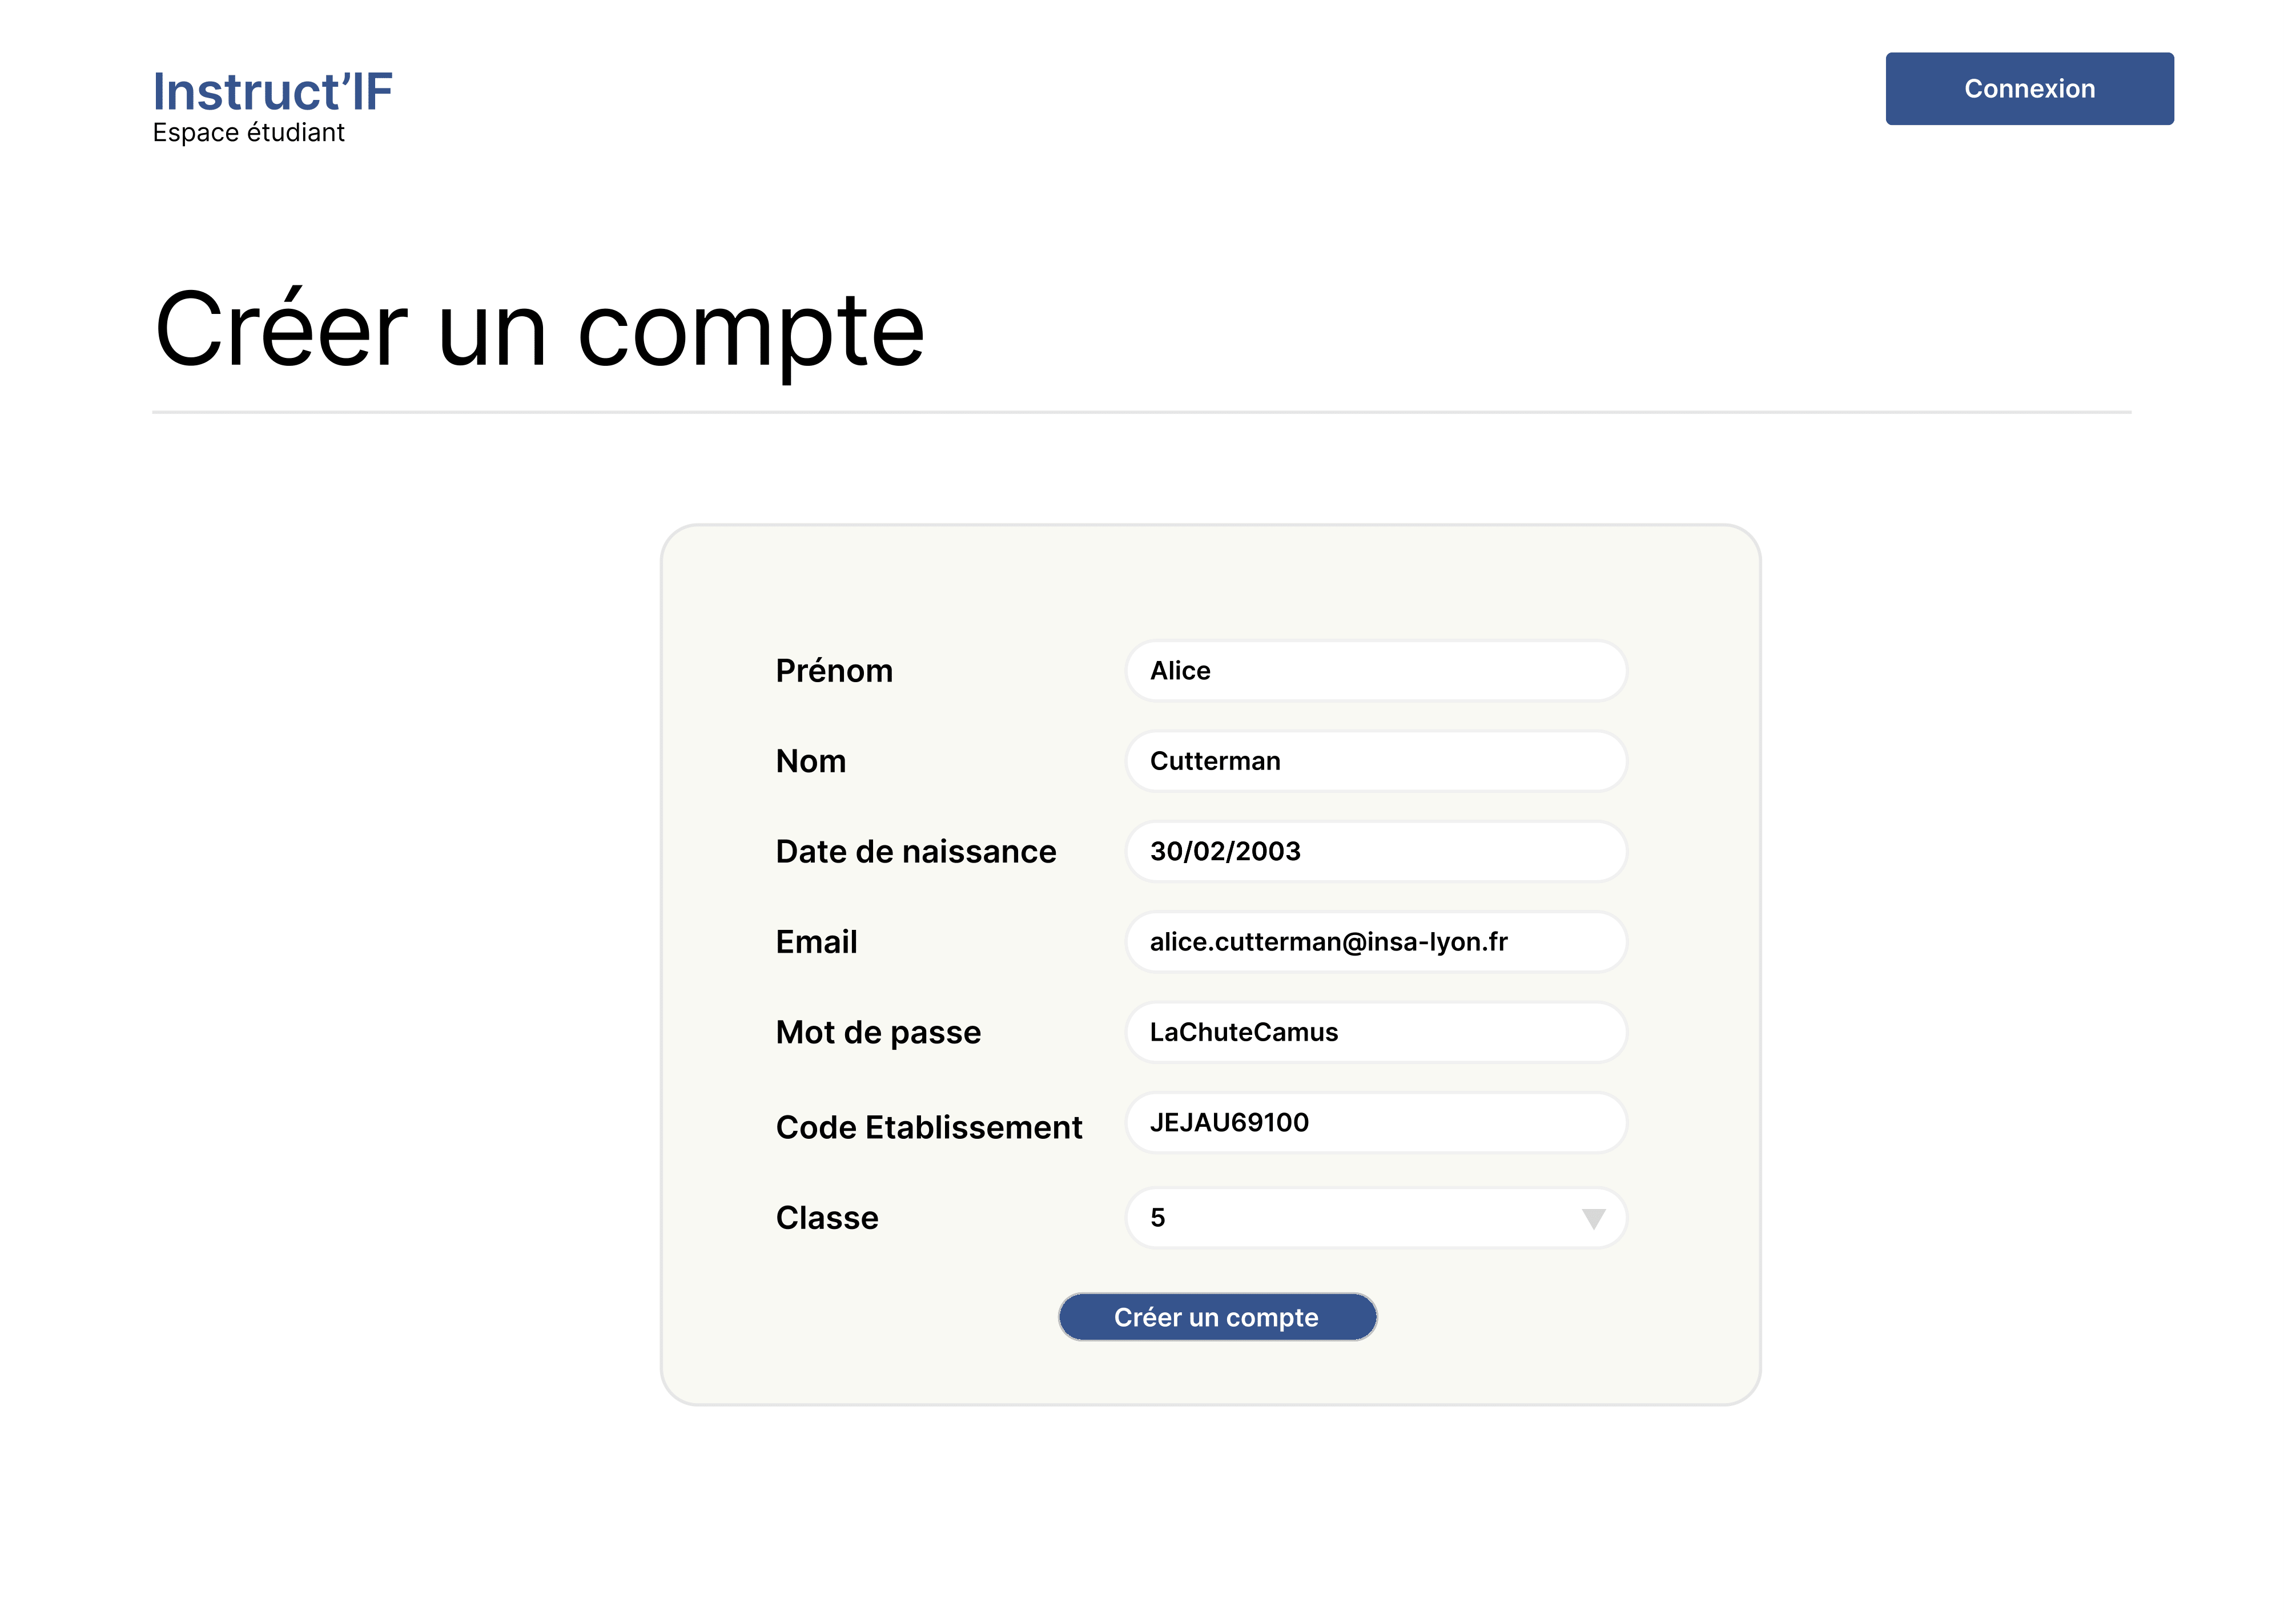
\includegraphics[width=11cm]{IHM/signinEleve.png}}
    \caption{Fenêtre de création de compte de (IHM Elève)}
\end{figure}

\begin{figure}[H]
    \centering
    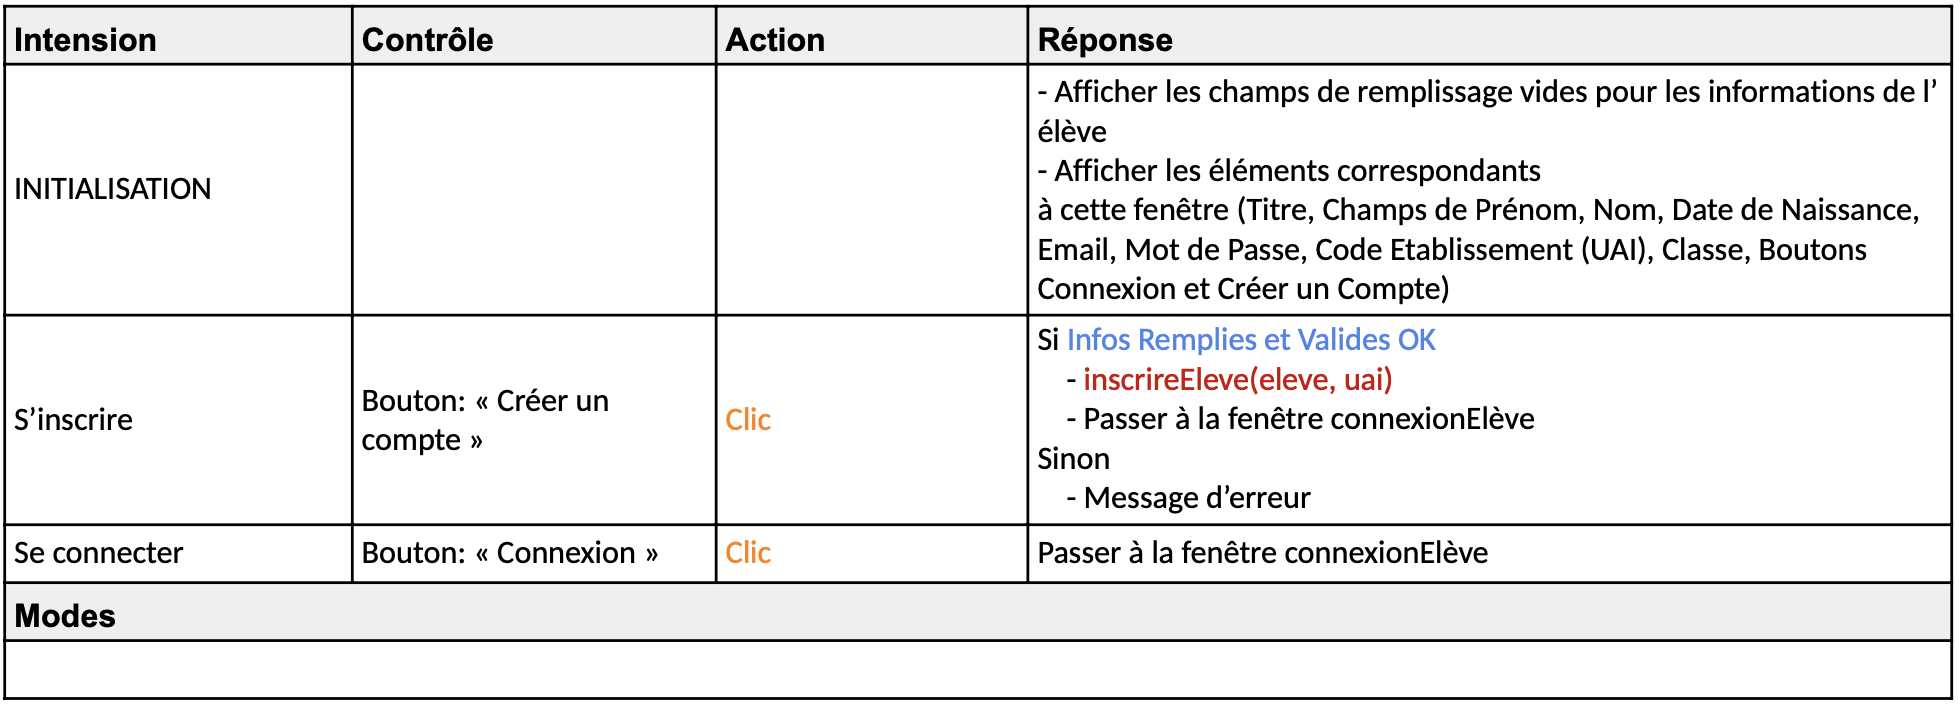
\includegraphics[width=13cm]{ICARS/inscription.png}
    \caption{ICAR+S associé à l'IHM de création de compte (IHM Elève)}
\end{figure}

\begin{figure}[H]
    \centering
    \fbox{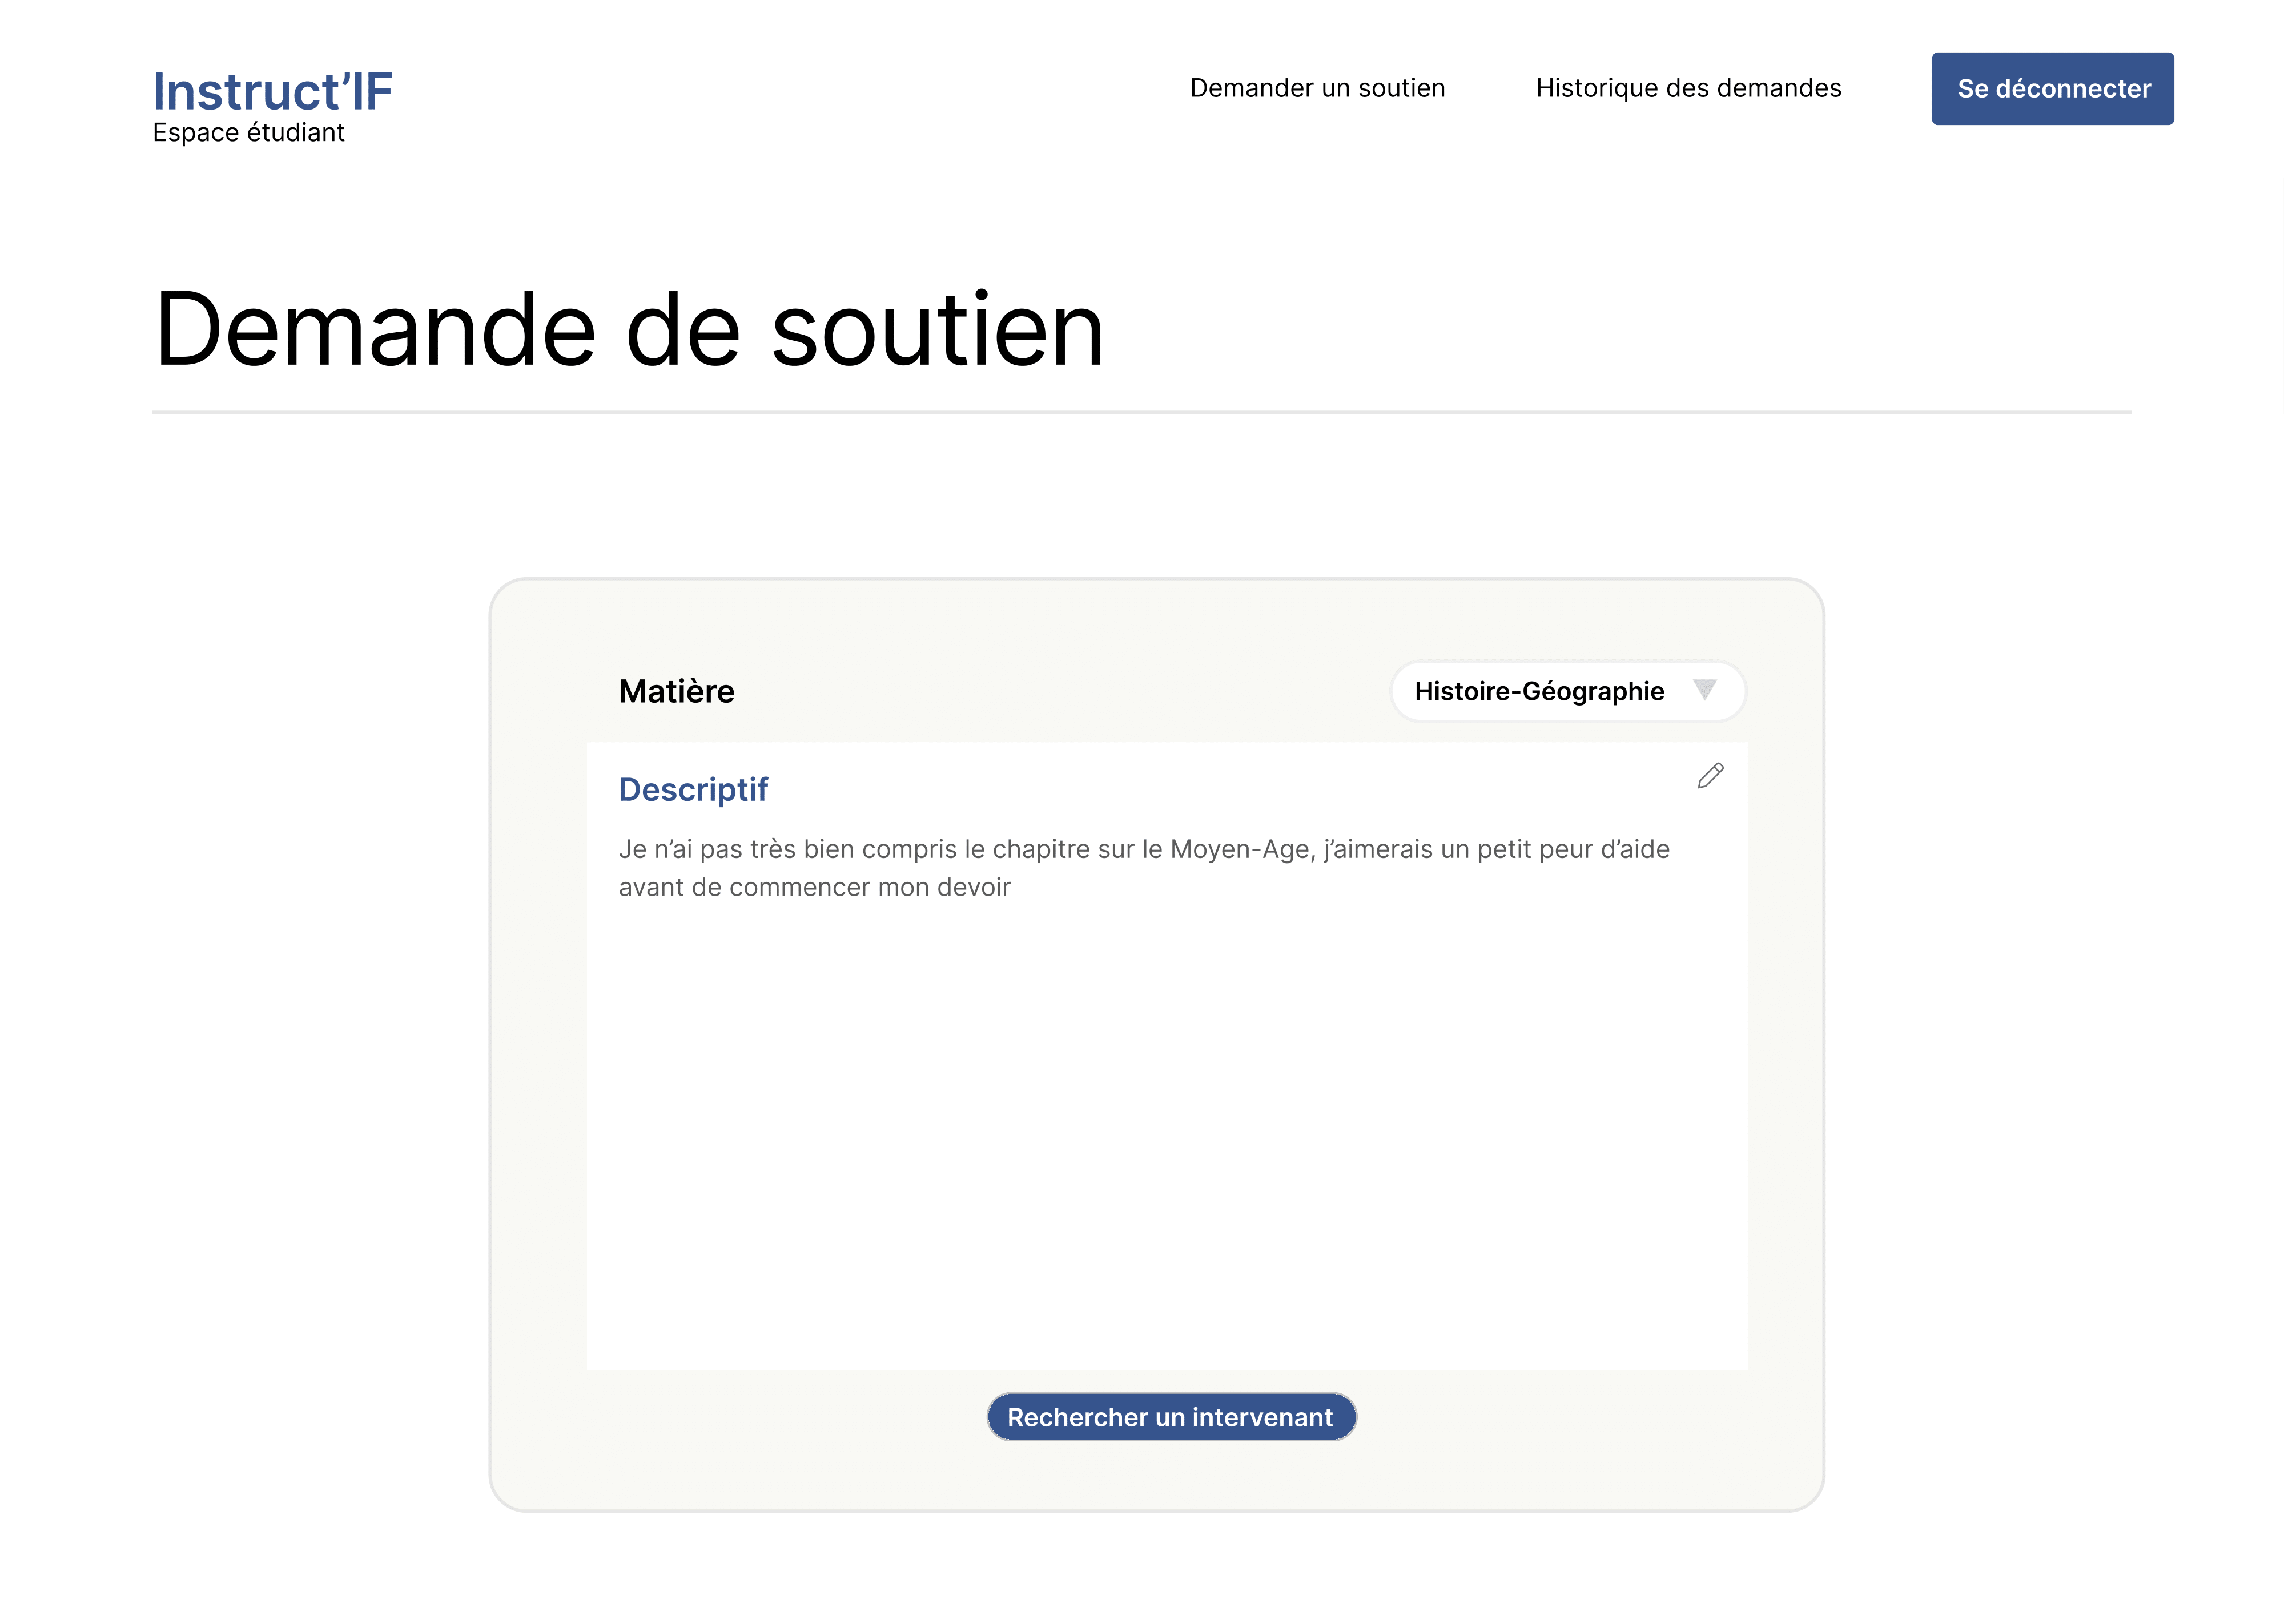
\includegraphics[width=11cm]{IHM/demandeEleve.png}}
    \caption{Fenêtre de demande de soutien (IHM Elève)}
\end{figure}

\begin{figure}[H]
    \centering
    \fbox{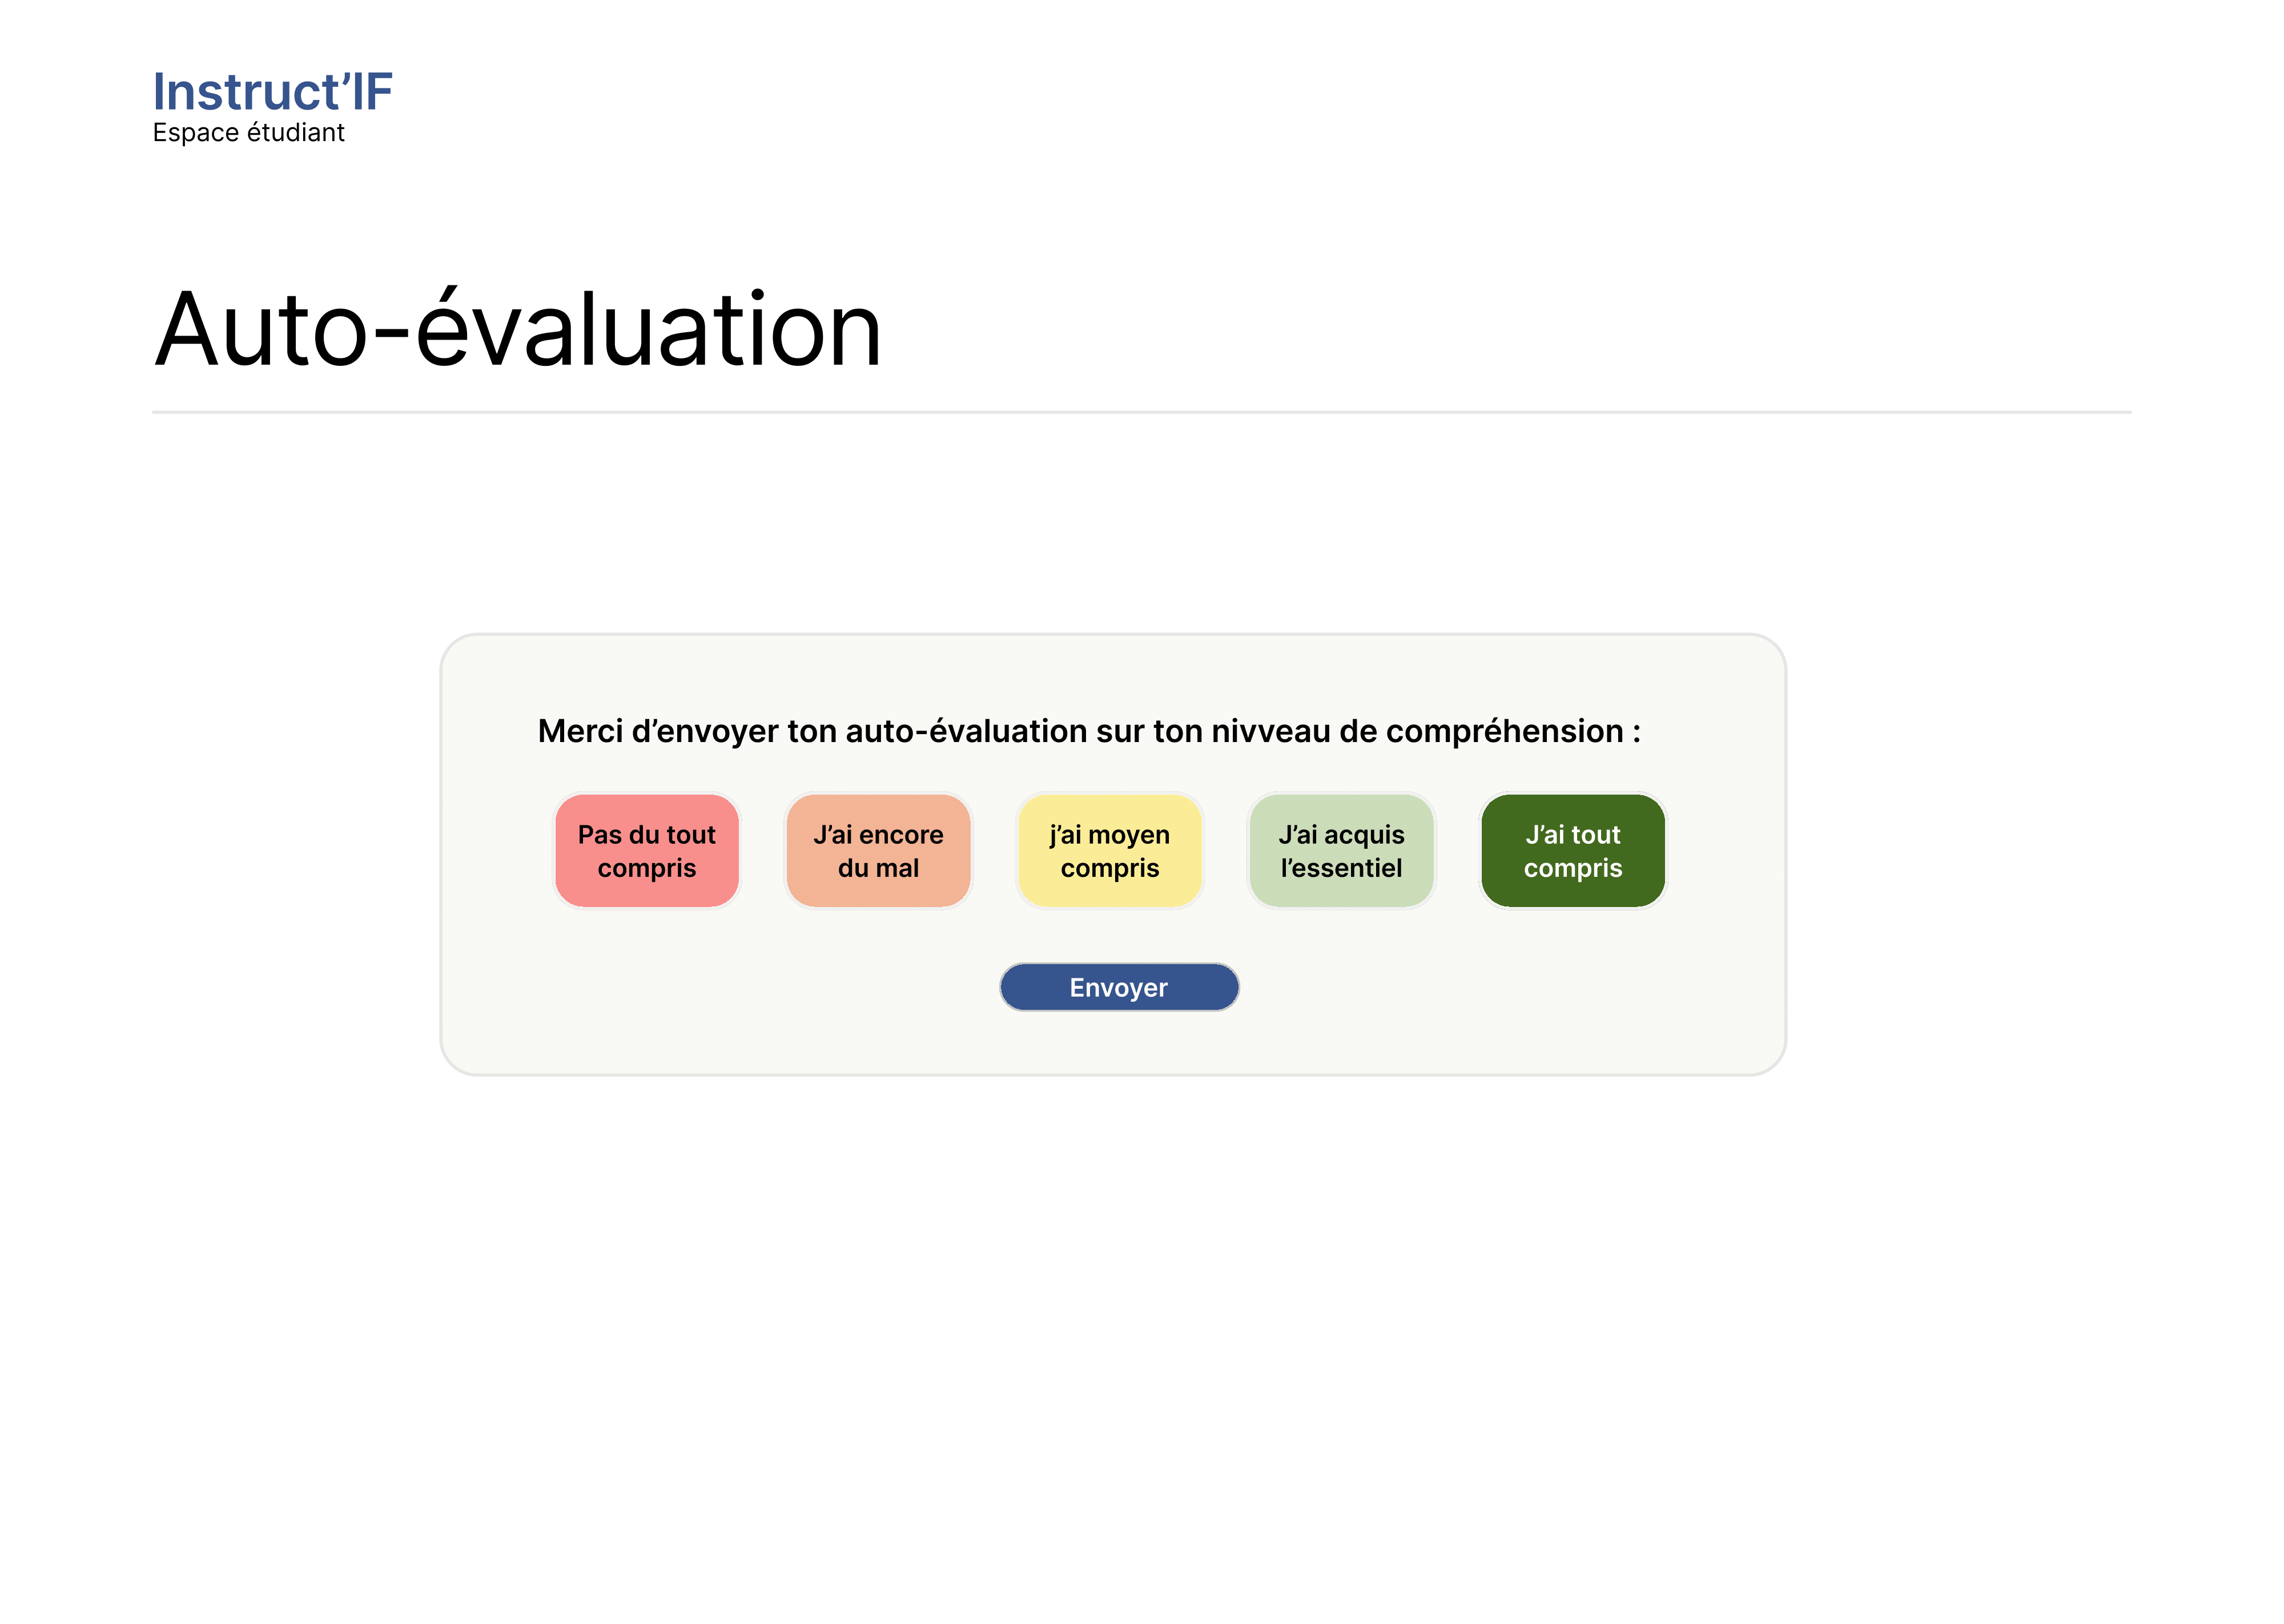
\includegraphics[width=11cm]{IHM/autoevaluation.png}}
    \caption{Fenêtre d'auto évaluation de l'élève (IHM Elève)}
\end{figure}

\begin{figure}[H]
    \centering
    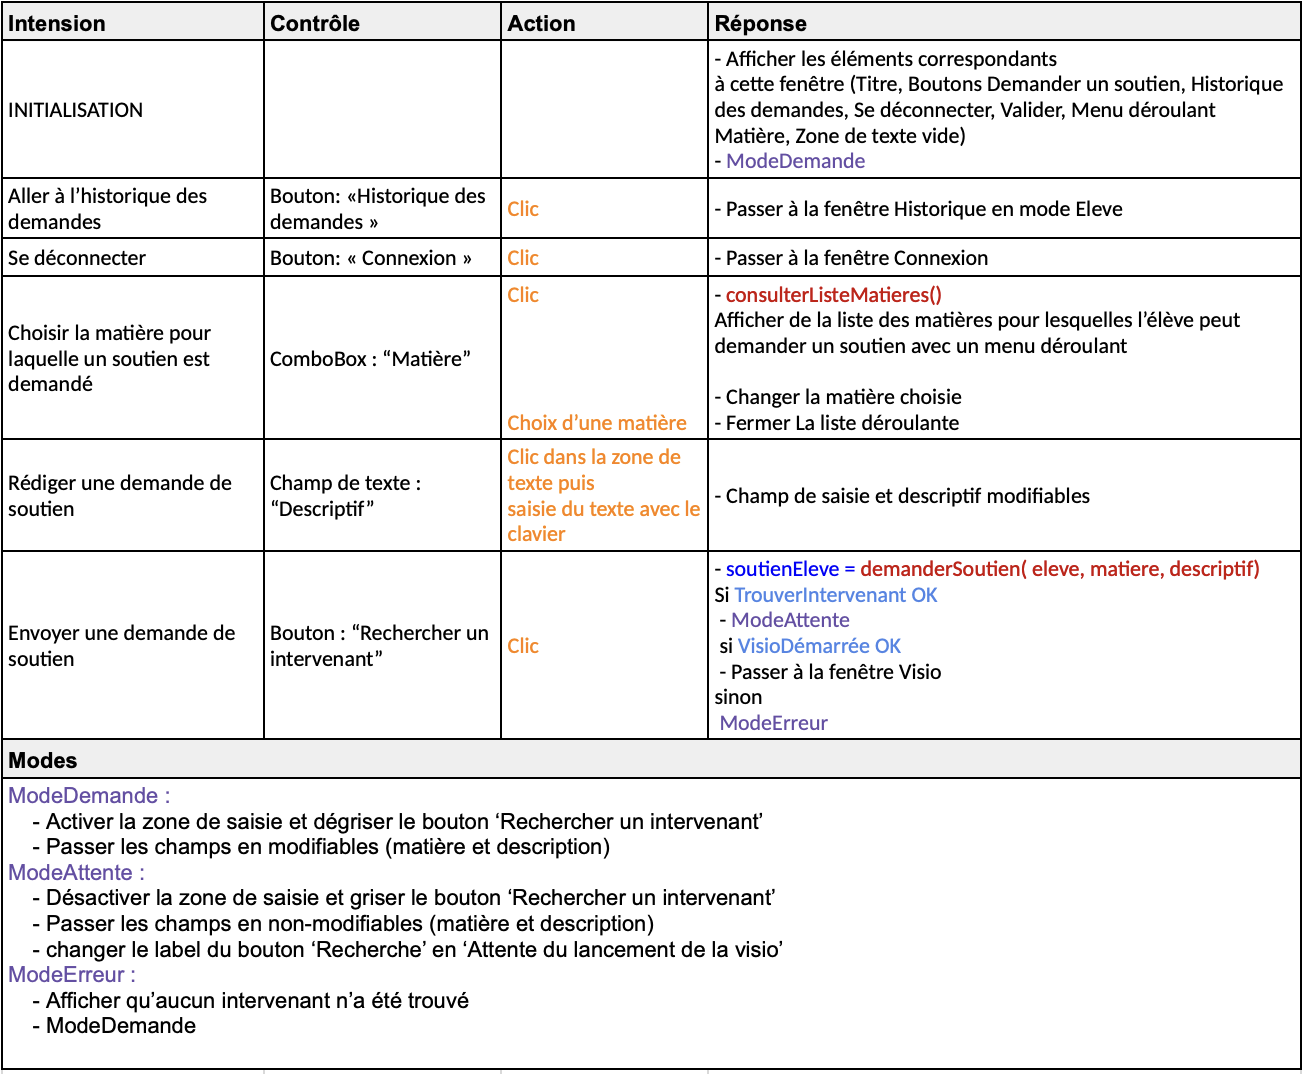
\includegraphics[width=13cm]{ICARS/demandeEleve.png}
    \caption{ICAR+S associé à l'IHM de demande de soutien (IHM Elève)}
\end{figure}

\begin{figure}[H]
    \centering
    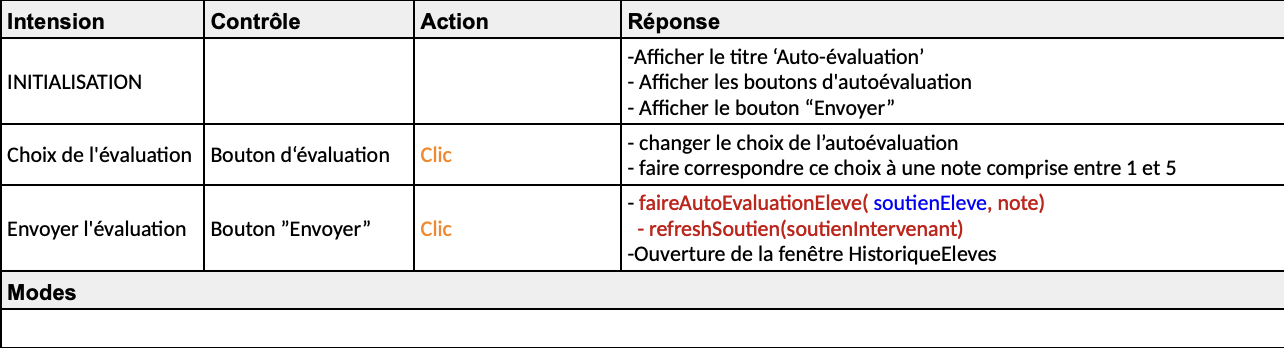
\includegraphics[width=13cm]{ICARS/autoeval.png}
    \caption{ICAR+S associé à l'IHM d'auto évaluation de l'élève (IHM Elève)}
\end{figure}


\subsection{IHM Intervenant}

\begin{figure}[H]
    \centering
    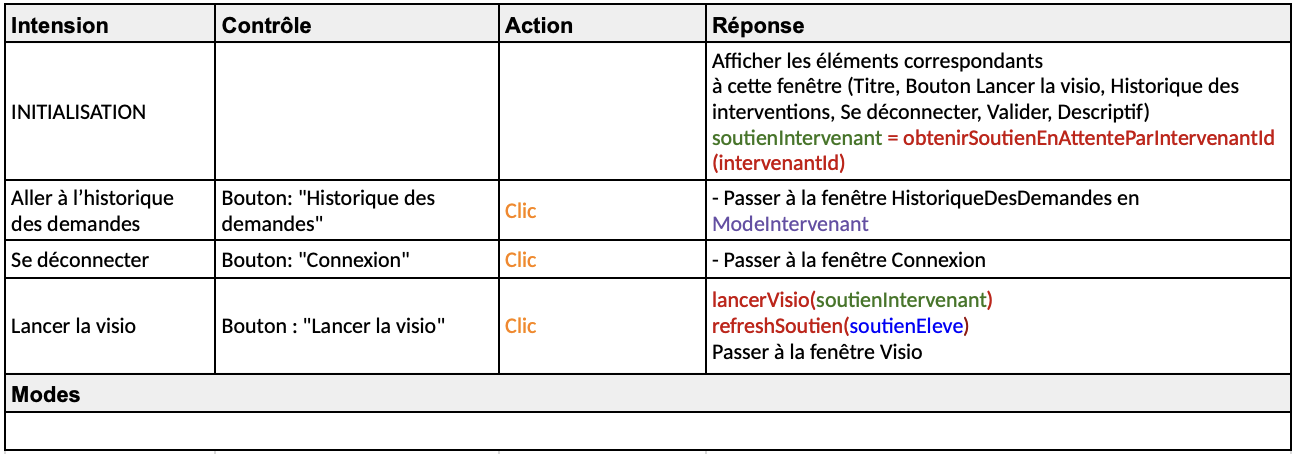
\includegraphics[width=13cm]{ICARS/demandeInter.png}
    \caption{ICAR+S associé à l'IHM de demande de soutien (IHM Intervenant)}
\end{figure}

\begin{figure}[H]
    \centering
    \fbox{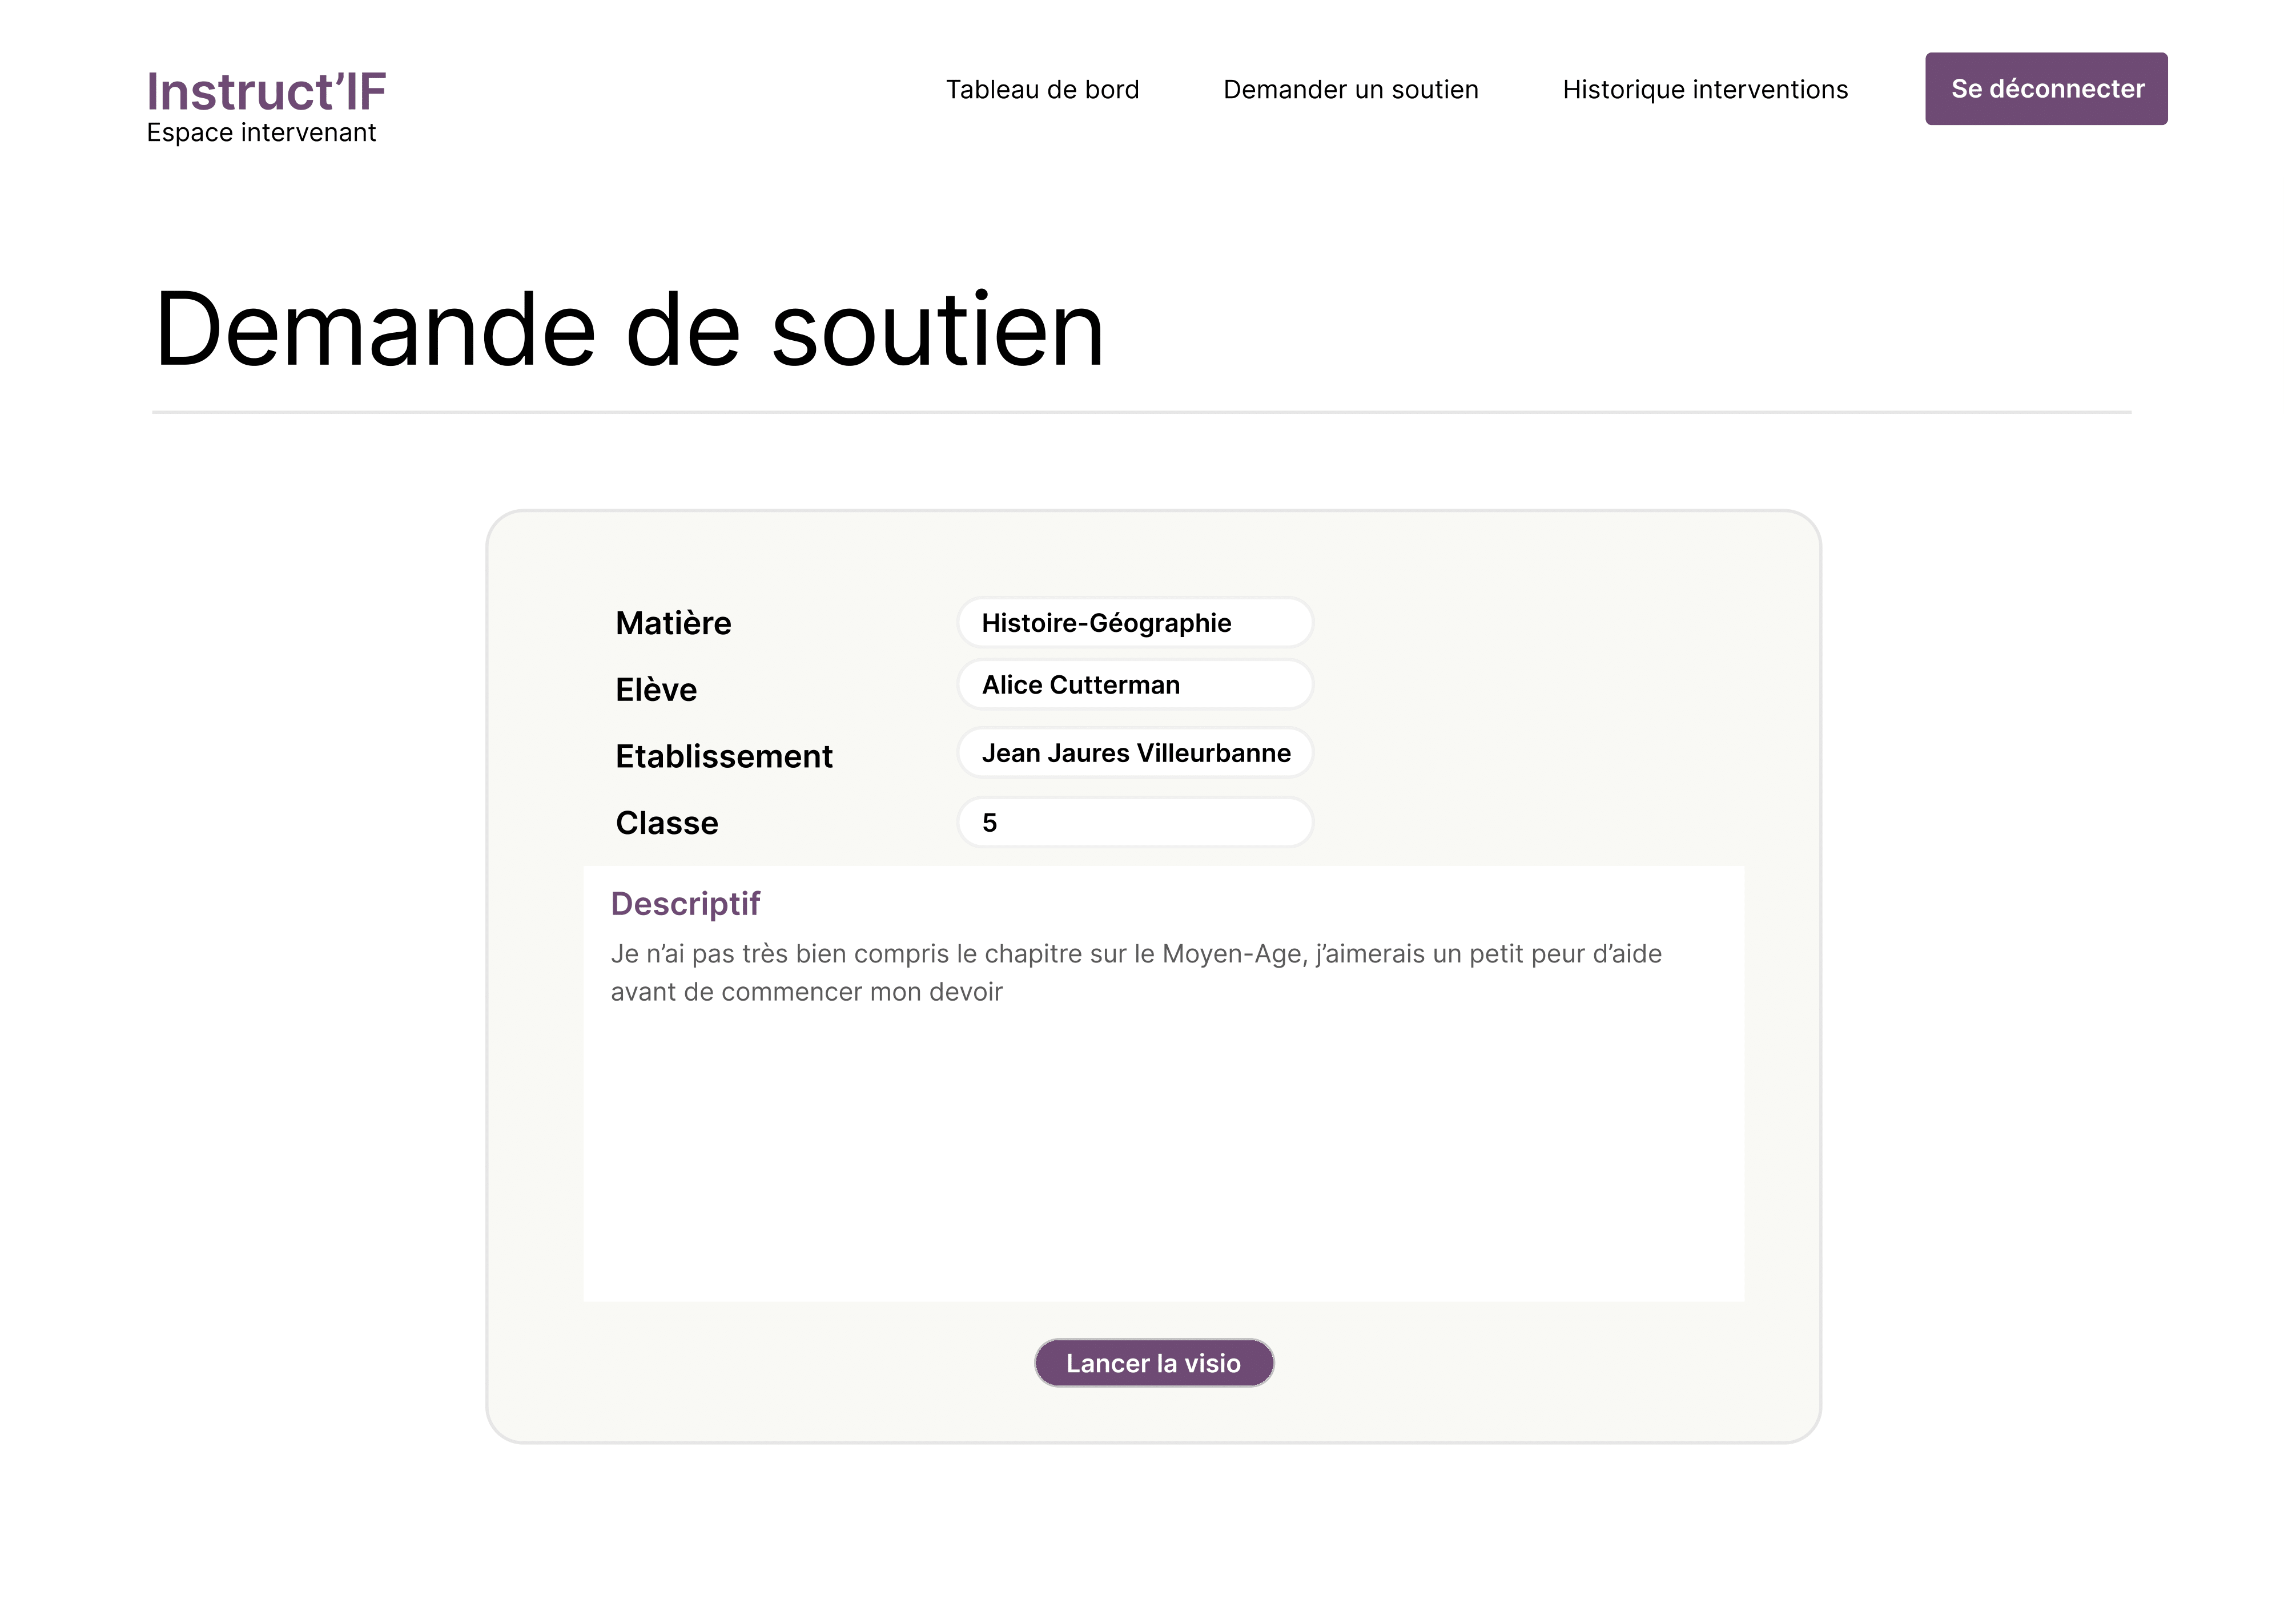
\includegraphics[width=11cm]{IHM/demandeIntervenant.png}}
    \caption{Fenêtre de demande de soutien (IHM Intervenant)}
\end{figure}


\begin{figure}[H]
    \centering
    \fbox{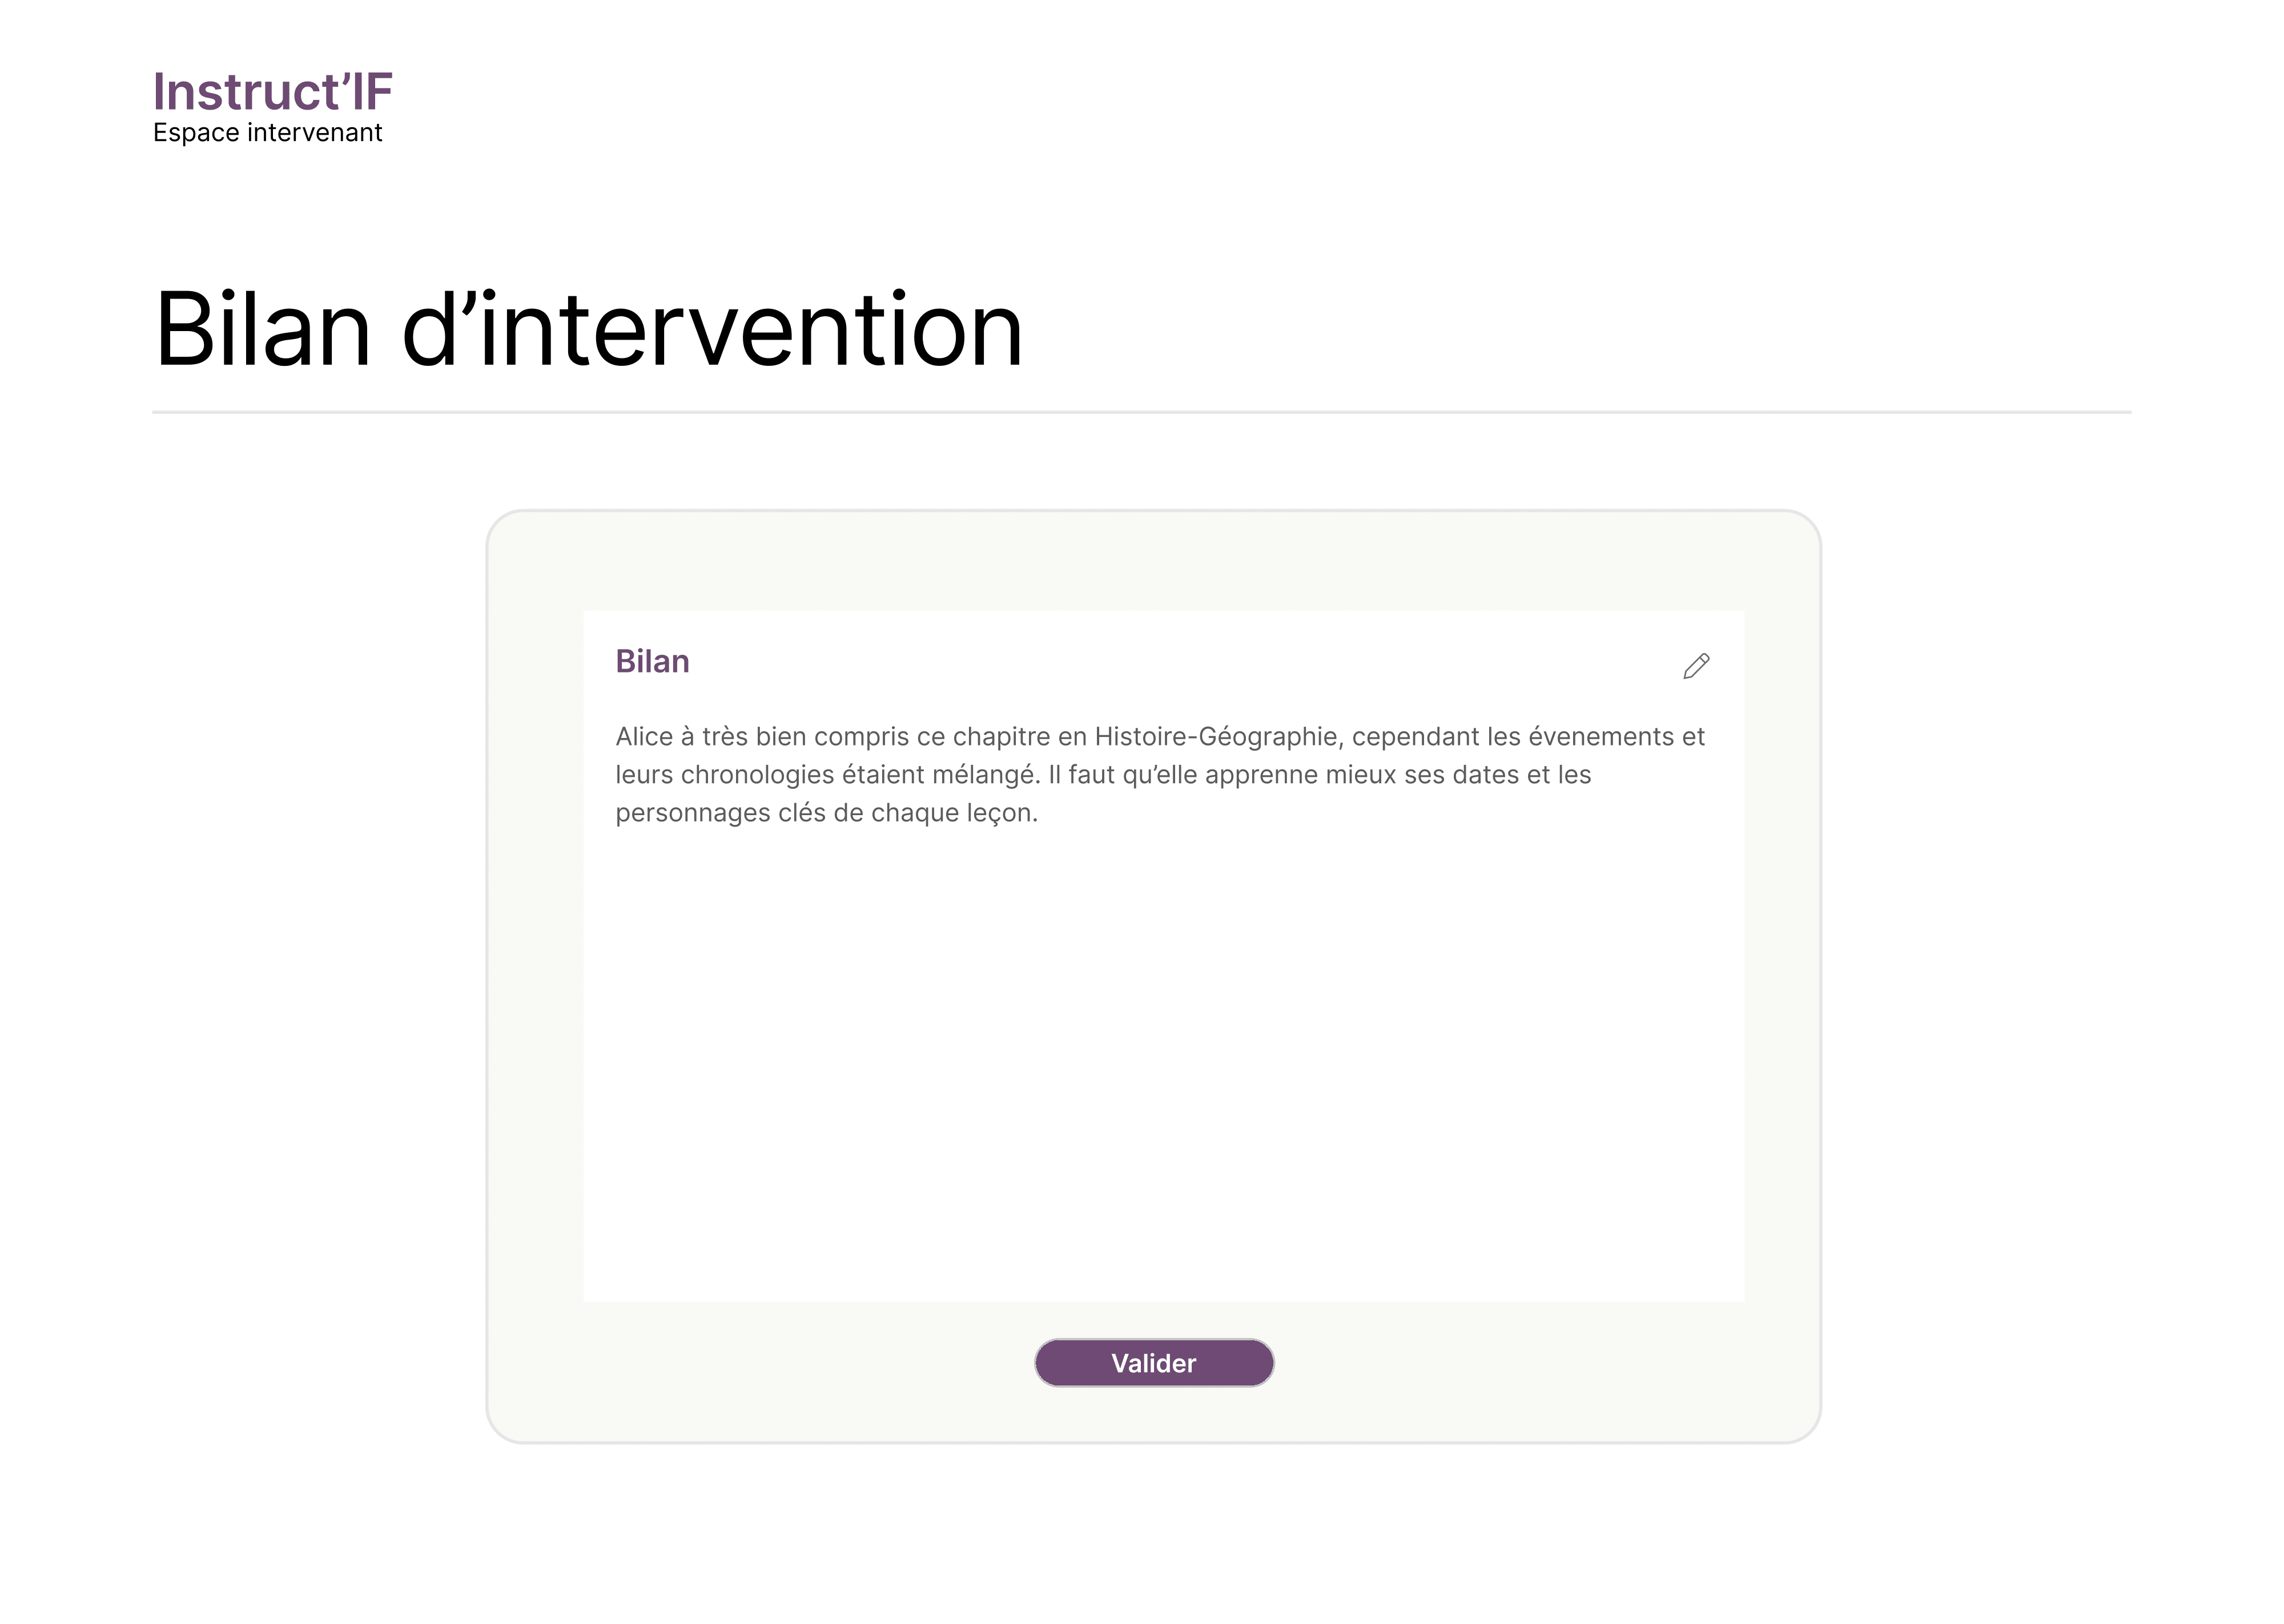
\includegraphics[width=11cm]{IHM/bilan.png}}
    \caption{Fenêtre de rédaction du bilan (IHM Intervenant)}
\end{figure}

\begin{figure}[H]
    \centering
    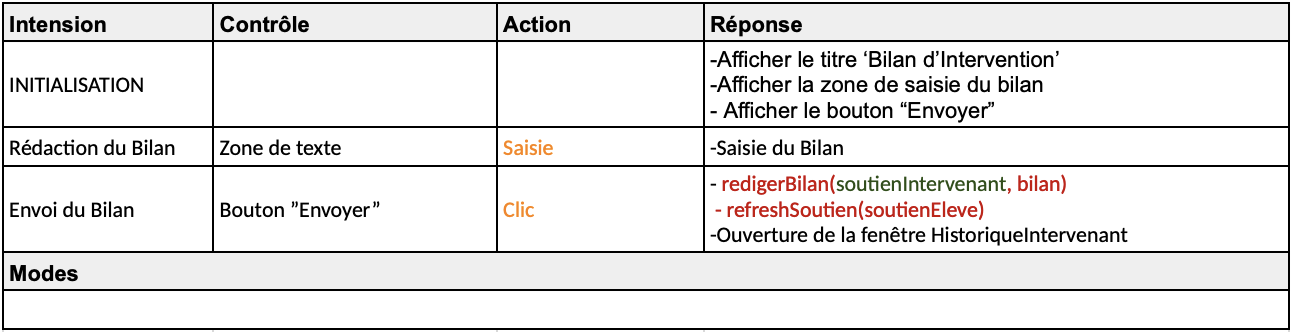
\includegraphics[width=13cm]{ICARS/redacBilan.png}
    \caption{ICAR+S associé à l'IHM de rédaction du bilan (IHM Intervenant)}
\end{figure}

\begin{figure}[H]
    \centering
    \fbox{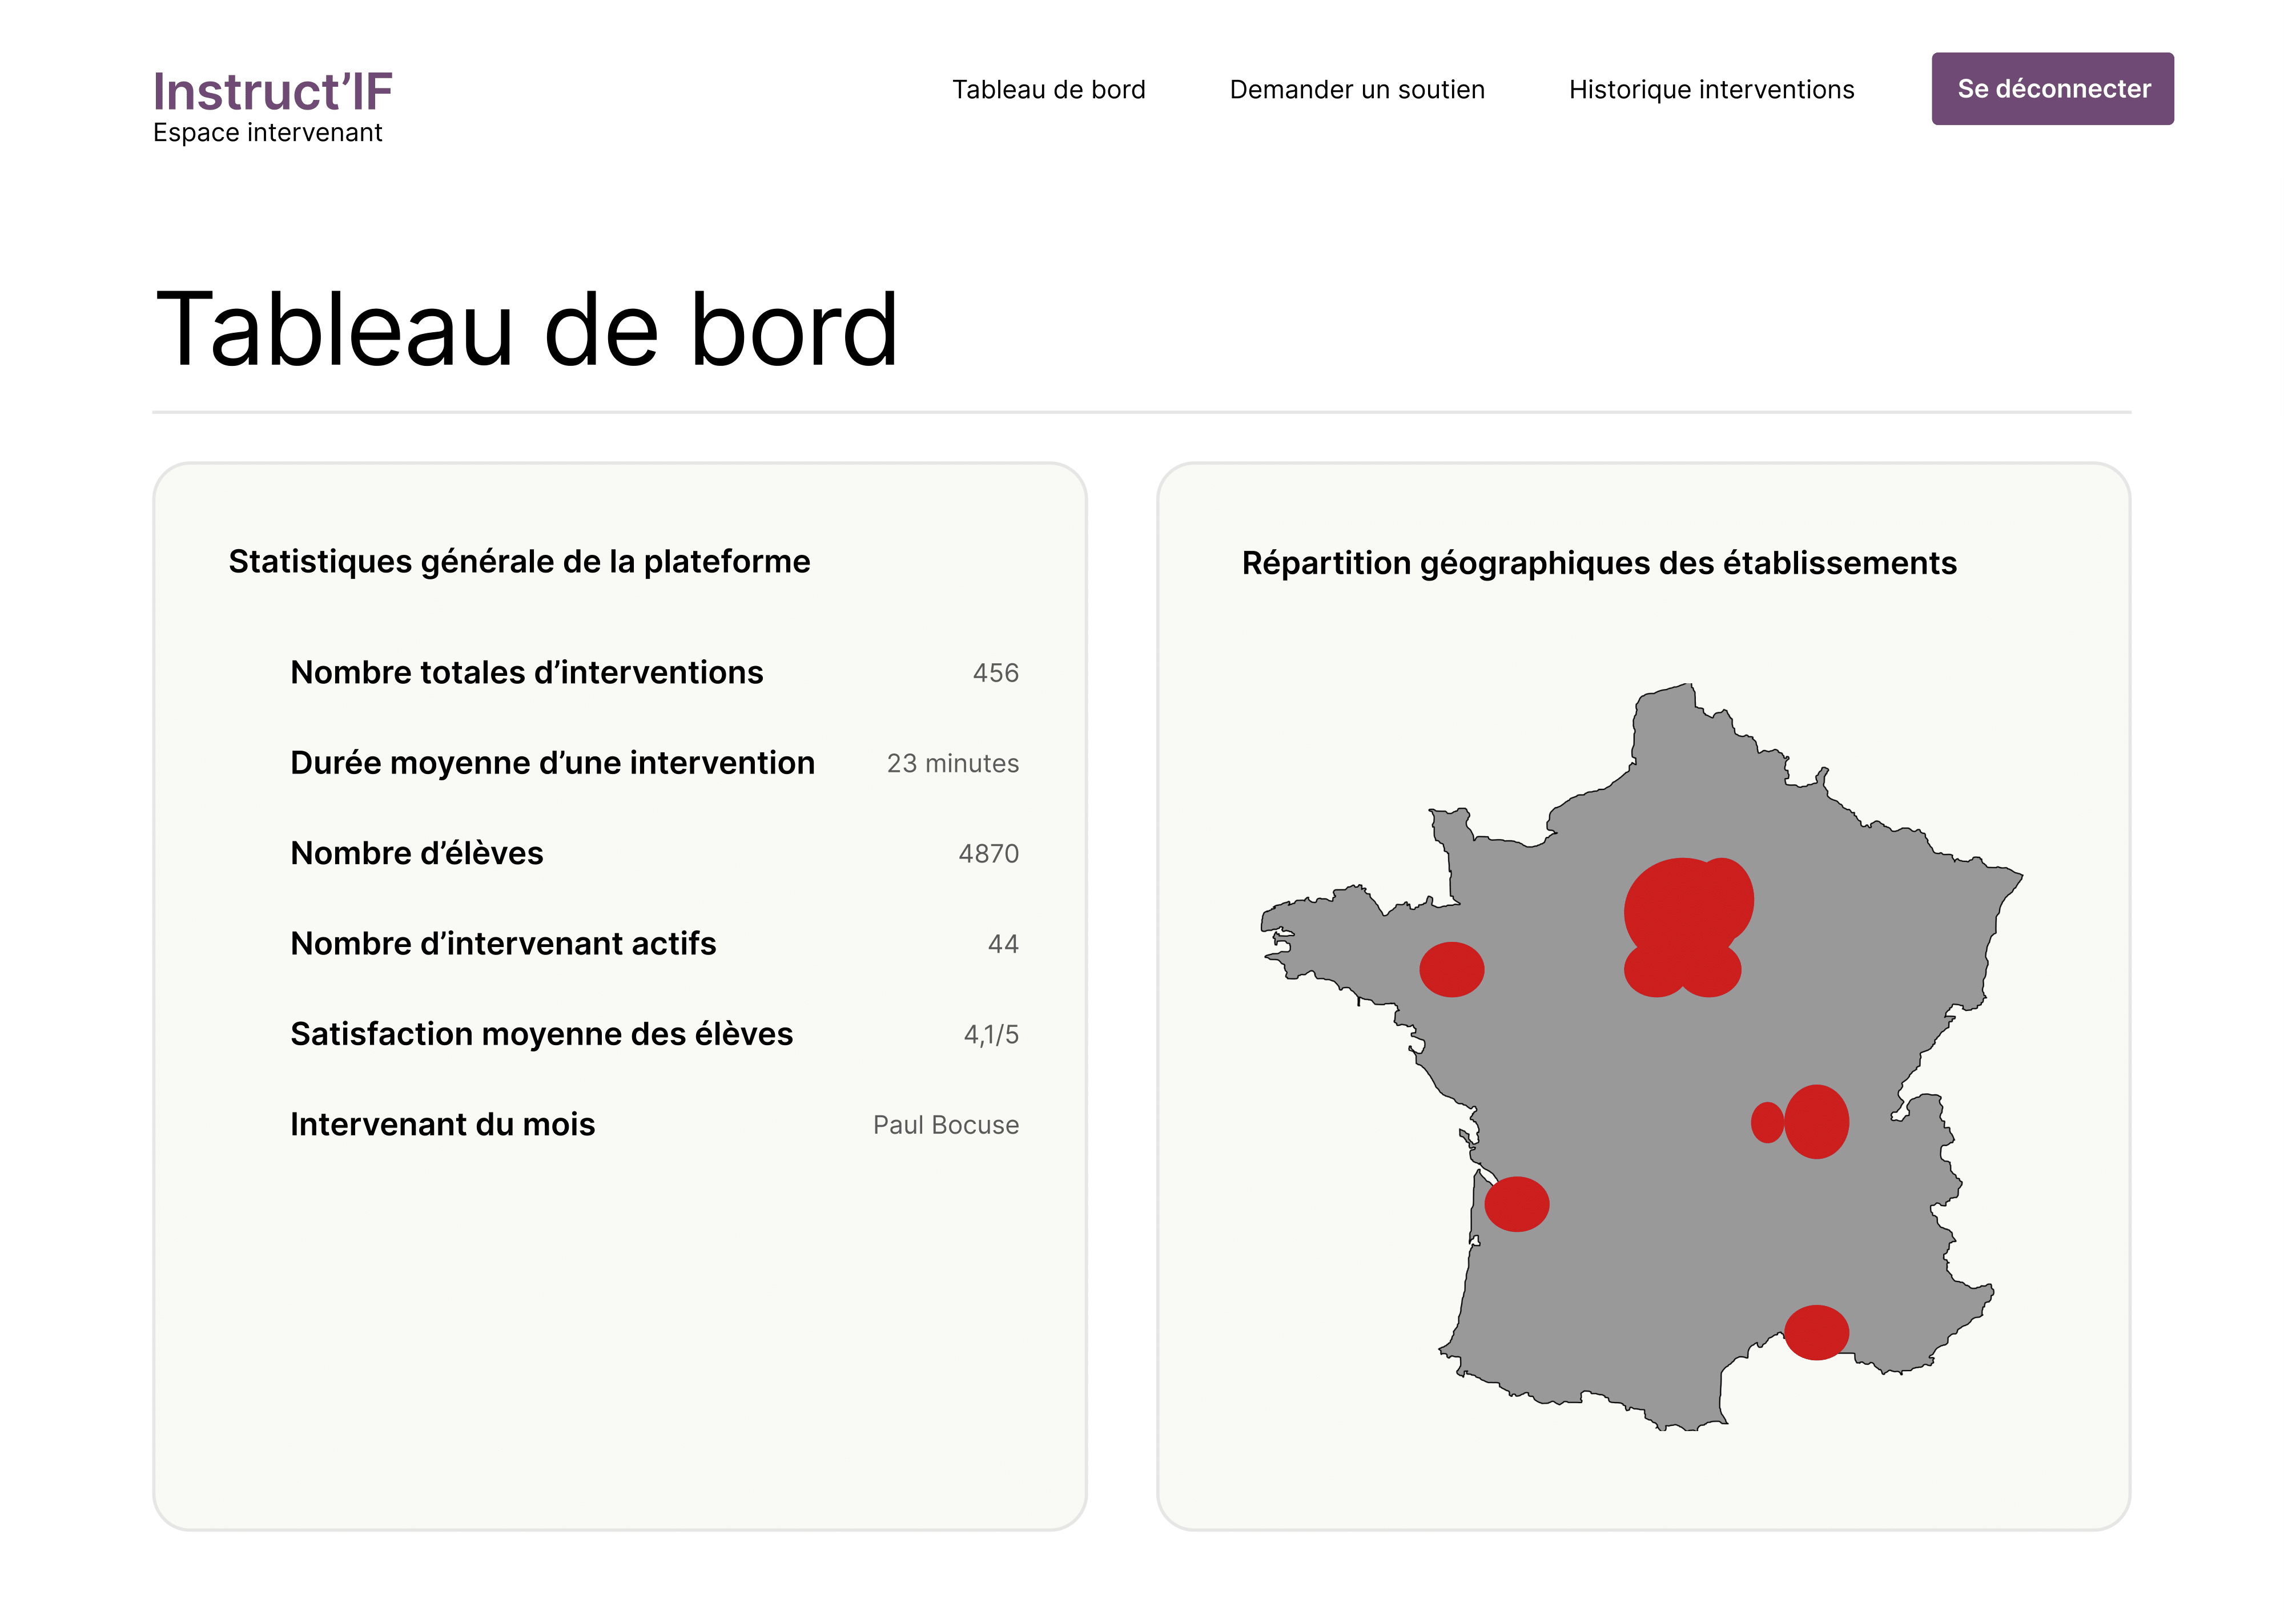
\includegraphics[width=11cm]{IHM/tdb.png}}
    \caption{Fenêtre du tableau de bord (IHM Intervenant)}
\end{figure}

\begin{figure}[H]
    \centering
    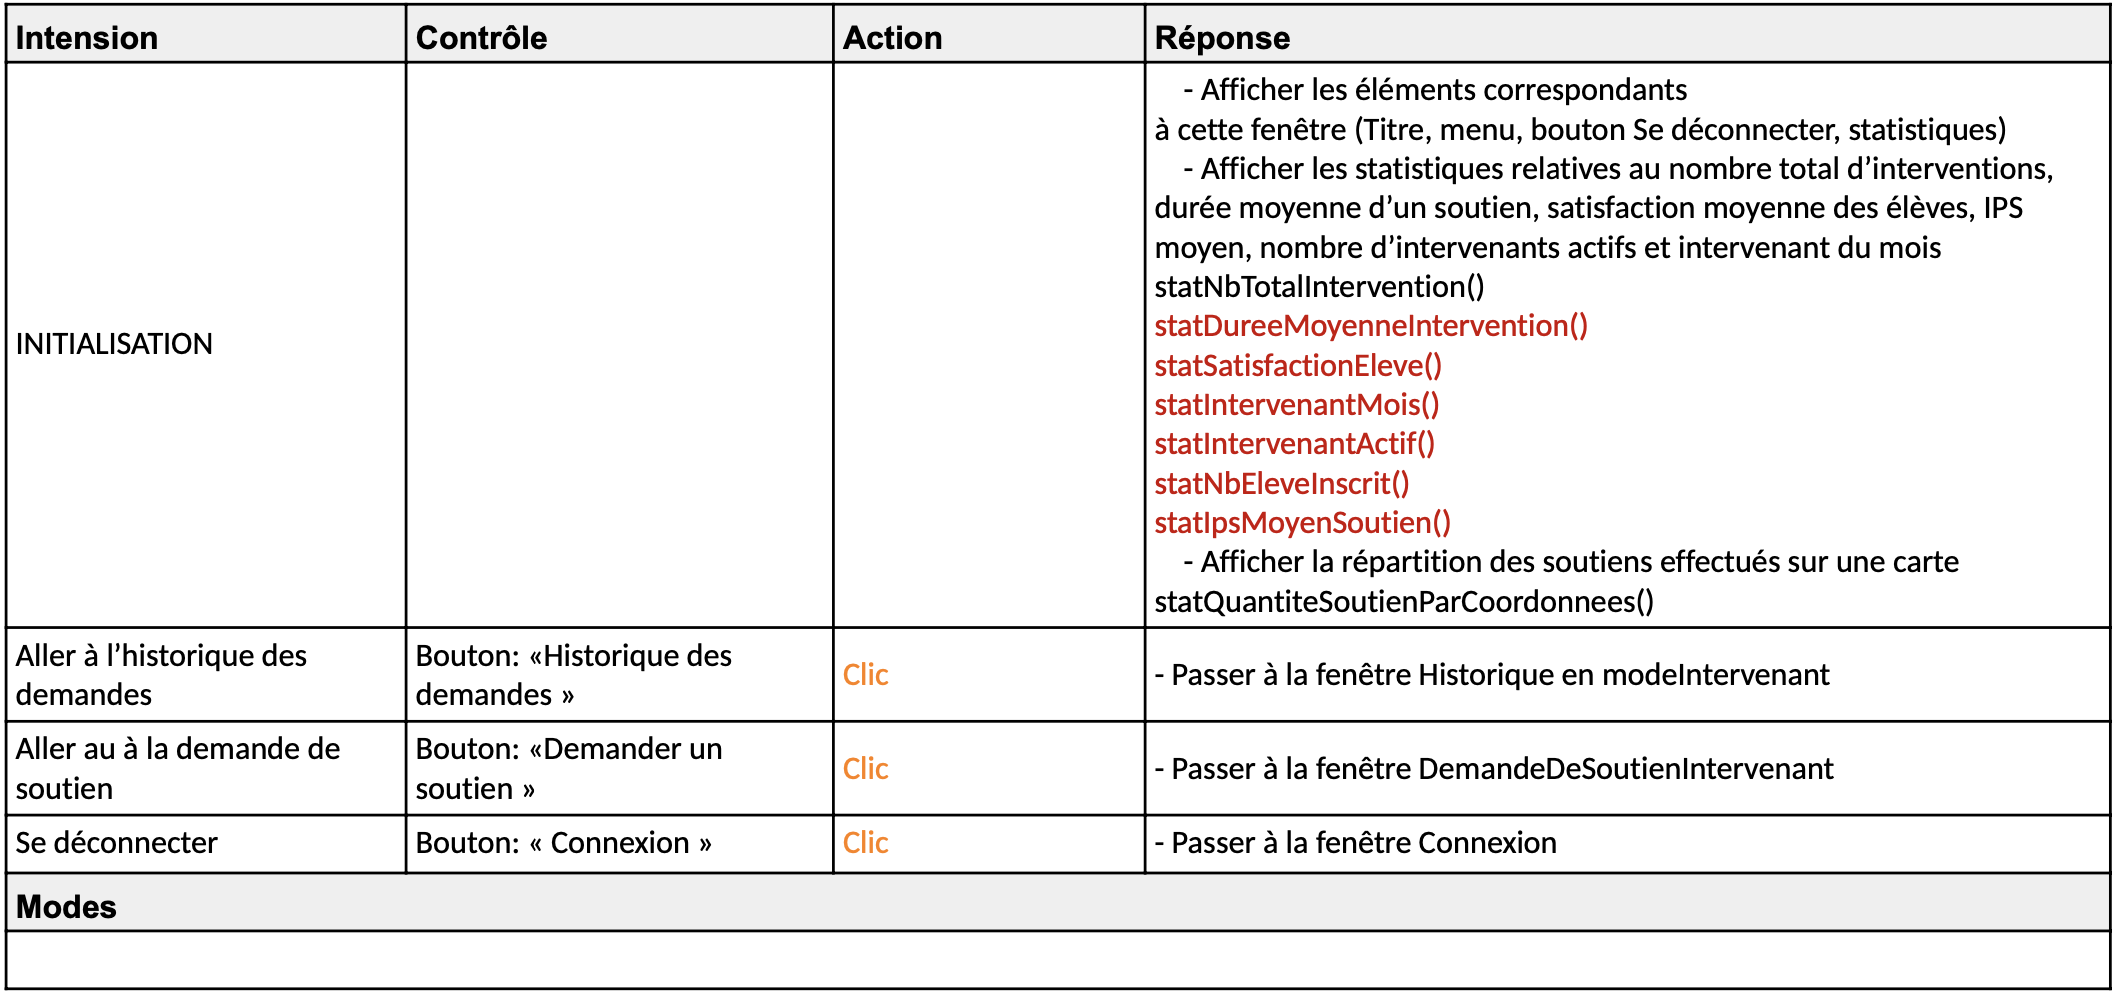
\includegraphics[width=13cm]{ICARS/tdb.png}
    \caption{ICAR+S associé à l'IHM du tableau de bord (IHM Intervenant)}
\end{figure}

\section{Spécification des services}

\subsection{Services d'initialisation}

\begin{lstlisting}[language = Java]
public void initialisation()
\end{lstlisting}

Nous avons fait le choix de regrouper la création en "dur" des intervenants ainsi que des matières dans un service d'initialisation. Cependant les services d'inscription des intervenants ainsi que des matières sont dans des services externes. Cela permet notamment d'enrichir les bases de données avec d'autres intervenants ou d'autres matières pour des extensions futures.

\begin{lstlisting}[language = Java]
public Boolean inscrireIntervenant(Intervenant intervenant)
\end{lstlisting}
\begin{lstlisting}[language = Java]
public Boolean creerMatiere(Matiere matiere)
\end{lstlisting}

\subsection{Services élèves}
\begin{lstlisting}[language = Java]
public Boolean inscrireEleve(Eleve eleve, String uai)
\end{lstlisting}
Ce service d'inscription d'élève réalise la persistance des élèves dans la base de données. Il commence par vérifier que l'établissement de l'élève qui a été renseigné à l'aide de son code uai est valide. Cette validation est réalisée à l'aide d'une API externe (EducNetApi), puis persiste en base de donnée, si cela n'est pas déjà fait, l'établissement.\\
Voici un pseudo code expliquant le déroulé de cet algorithme : 
\begin{lstlisting}[language =]
fonction inscrireEleve(eleve, uai) {
    creer le contexte de persistance avec JpaUtil
    
    si EducNetApi confirme l'existence de l'etablissement avec uai {
        si l'etablissement n'existe pas dans notre base {
            creer un nouvel etablissement avec ces informations via EducNetApi
            obtenir latitude et longitude de l'etablissement via GeoNetApi
            persister le nouvel etablissement
        }
        sinon {
            recuperer l'etablissement existant de notre base
        }
        associer l'eleve a l'etablissement
        persister l'eleve
        valider la transaction
        envoyer un mail de confirmation a l'eleve
        }
    si echec {
        annuler la transaction
        envoyer un mail d'echec a l'eleve
    }
}
\end{lstlisting}

\begin{lstlisting}[language = Java]
public Eleve authentifierEleveMail(String mail, String motDePasse)
\end{lstlisting}
Ce service permet aux élèves de s'authentifier à l'aide de leur mail ainsi que leur mot de passe. Il fait appel à la méthode \texttt{getParMail} de la classe \texttt{eleveDao} qui retourne l'élève avec le mail associé et compare les mots de passe. Si le mot de passe est correct, ce service retourne l'élève.

\begin{lstlisting}[language = Java]
public List<Soutien> trouverHistoriqueEleve(Eleve eleve)
\end{lstlisting}
Ce service retourne une liste d'objets soutien. Ces objets sont tous les soutiens réalisé par l'élève passé en paramètre.


\subsection{Services intervenants}
\begin{lstlisting}[language = Java]
public Intervenant authentifierIntervenantTelephone(String telephone, String motDePasse)
\end{lstlisting}
Ce service permet aux intervenants de s'authentifier à l'aide de leur numéro de téléphone ainsi que leur mot de passe. Il va faire appel à la méthode \texttt{getParTelephone} de la classe \texttt{intervenantDao} qui retourne l'intervenant avec le numéro de téléphone associé et compare les mot de passe. Si le mot de passe est correct, ce service retourne l'intervenant.

\begin{lstlisting}[language = Java]
public List<Soutien> trouverHistoriqueIntervenant(Intervenant intervenant)
\end{lstlisting}
Ce service retourne une liste d'objets soutien. Ces objets sont tous les soutiens supervisés par l'intervenant passé en paramètre.

\subsection{Services soutiens}
Lorsqu'un élève souhaite demander un soutien, il remplit les informations nécessaires puis demande le soutien avec le service \texttt{demanderSoutien}.
\begin{lstlisting}[language = Java]
public Soutien demanderSoutien(Eleve eleve, Matiere matiere, String descriptif)
\end{lstlisting}
Ce service permet de persister un soutien d'un élève. Il prend en paramètre l'élève qui à fait la demande, la matière sélectionnée à l'aide du service \texttt{consulterListeMatiere} ainsi que le descriptif renseigné par l'élève. Cette méthode va notamment faire appel aux setter de la classe \texttt{Soutien} pour définir ses attributs. La méthode \texttt{trouverIntervenantSoutien} décrite postérieurement sélectionne un intervenant puis l'associe au soutien. Une notification est finalement envoyée à l'intervenant pour l'informer de son soutien en attente.
\begin{lstlisting}[language =]
fonction demanderSoutien(eleve, matiere, descriptif) {
    creer le contexte de persistance avec JpaUtil
    creer un nouvel objet Soutien
      
    definir l'eleve, le descriptif et la matiere du soutien
    trouver un intervenant pour le soutien avec la methode trouverIntervenantSoutien
    si aucun intervenant n'a ete trouve {
        envoyer un mail de rejet de la demande et sortir de la methode en envoyant une exception }
    sinon {
        assigner cet intervenant au soutien} 
    mettre a jour la disponibilite et le nombre d'interventions de l'intervenant
      
    ouvrir une transaction
    mettre a jour l'intervenant dans la base de donnees
    persister l'objet Soutien dans la base de donnees
    valider la transaction
      
    envoyer une notification a l'intervenant pour lui signaler la prise en charge de la demande
    
    si ehcec {
      afficher l'erreur
      annuler la transaction
      envoyer un mail a l'eleve pour signaler l'echec de la demande
    }
    fermer le contexte de persistance
    retourner l'objet Soutien
}
\end{lstlisting}

\begin{lstlisting}[language = Java]
public List<Matiere> consulterListeMatieres()
\end{lstlisting}
Service permettant d'obtenir la liste des matières disponible sur l'application.

\begin{lstlisting}[language = Java]
public Intervenant trouverIntervenantSoutien(Eleve eleve)
\end{lstlisting}
Ce service sélectionne un intervenant selon les critères exigés dans le cahier des charges. En premier lieu nous créons une liste de tous les intervenants puis les trions par ordre croissant de nombre d'interventions réalisées. Nous parcourons ensuite cette liste et sélectionnons le premier qui vérifie les conditions de disponibilité ainsi que de niveau académique compatible avec l'élève.

\begin{lstlisting}[language =]
fonction trouverIntervenantSoutien(Eleve eleve) {      
    cree une liste de tous les intervenants
    trie cette liste par ordre croissant de nombre d'intervention
    pour chaque intervenant de la liste {
        si disponiblite == true && niveauMin < classeEleve < niveauMax {
            selectionne cet intervenant
            break
        }
    }
    retourne intervenant selectionne
}
\end{lstlisting}

\begin{lstlisting}[language = Java]
public Soutien obtenirSoutienEnAttenteParEleveId(Long eleveId)
public Soutien obtenirSoutienEnAttenteParIntervenantId(Long intervenantId)
\end{lstlisting}
Ces deux services renvoient les soutiens en attente d'un intervenant et d'un élève dont l'id est rentré en paramètre.

\begin{lstlisting}[language = Java]
public Boolean lancerVisio(Soutien soutien)
\end{lstlisting}
Ce service permet de lancer la visioconférence. Elle vérifie tout d'abord qu'un intervenant à bien été sélectionné puis met à jour l'état pour qu'il passe à " \texttt{EN VISIO} " et renseigne également la date de début de la visioconférence.

\begin{lstlisting}[language = Java]
public Boolean terminerVisio(Soutien soutien)
\end{lstlisting}
Ce service permet de mettre fin à la visioconférence. Elle met à jour l'état pour qu'il passe à " \texttt{TERMINE} " et renseigne également la durée de la visioconférence. Ce service repasse également la disponibilité de l'intervenant à \texttt{true}.
\begin{lstlisting}[language = Java]
public Boolean faireAutoEvaluationEleve(Soutien soutien, Integer note)
\end{lstlisting}
Service permettant à l'élève de s'autoévaluer sur sa compréhension au terme de la visio. Cette note est ensuite utilisée pour calculer la satisfaction des élèves.

\begin{lstlisting}[language = Java]
public Boolean redigerBilan(Soutien soutien, String bilan)
\end{lstlisting}
Service permettant aux intervenant de réaliser un bilan de l'intervention à la suite de la visio. Ce bilan est ensuite envoyé par mail à l'élève mais aussi disponible dans l'historique des soutiens.

\begin{lstlisting}[language = Java]
public Soutien refreshSoutien(Soutien soutien)
\end{lstlisting}
Service permettant de rafraîchir l'état des entités Soutien avec leur représentation actuelle dans la base de données. Cela signifie que si des modifications ont été apportées à l'entité Soutien dans la base de données par d'autres transactions depuis le moment où il a été récupéré ou la dernière fois qu'il a été rafraîchie, ces modifications seront reflétées dans l'instance de l'entité après l'appel de refreshSoutien(soutien). Par exemple, si c'est l'intervenant qui a lancé la visio, la méthode lancerVisio(soutien\_intervenant) va changer l'état du soutien dans l'instance soutien\_intervenant mais pas dans l'objet soutien\_eleve. Il faut alors appeler refreshSoutien(soutien\_eleve) pour que l'objet soutien\_eleve soit à jour et conforme à l'entité Soutien de la base de données.

\subsection{Services statistiques}
Ces services sont utilisés pour réaliser les statistiques du tableau de bord visible dans l'IHM intervenant. Ils permettent notamment d'obtenir le nombre total d'intervention sur la plateforme tout intervenant confondus, la durée moyenne d'une intervention, la satisfaction des élèves, l'intervenant du mois, le nombre d'intervenant actifs et d'élèves inscrits. Nous pouvons également obtenir la satisfaction moyenne des élèves et enfin la répartition géographique des interventions.
\begin{lstlisting}[language = Java]
public Long statNbTotalIntervention()
\end{lstlisting}

\begin{lstlisting}[language = Java]
public Double statDureeMoyenneIntervention()
\end{lstlisting}

\begin{lstlisting}[language = Java]
public Double statSatisfactionEleve()
\end{lstlisting}

\begin{lstlisting}[language = Java]
public String statIntervenantMois()
\end{lstlisting}

\begin{lstlisting}[language = Java]
public Long statIntervenantActif()
\end{lstlisting}

\begin{lstlisting}[language = Java]
public Long statNbEleveInscrit()
\end{lstlisting}

\begin{lstlisting}[language = Java]
public Double statIpsMoyenSoutien()
\end{lstlisting}

\begin{lstlisting}[language = Java]
public List<List<Object>> statQuantiteSoutienParCoordonnees()
\end{lstlisting}

Ce dernier service retourne une List de List contenant des Object. Chaque List interne représente un ensemble de données où chaque élément correspond à :
\begin{itemize}
    \item La longitude de l'établissement (convertie en Double),
    \item La latitude de l'établissement (convertie en Double),
    \item Le nombre de soutiens associés à ces coordonnées géographiques (converti en Integer).
\end{itemize}
La fonction utilise une requête JPQL pour grouper les soutiens par les coordonnées géographiques des établissements des élèves et compter le nombre de soutiens pour chaque groupe de coordonnées. Les résultats de la requête sont ensuite organisés dans une structure de liste de listes pour être retournés.


\end{document}